% The document class supplies options to control rendering of some standard
% features in the result.  The goal is for uniform style, so some attention 
% to detail is *vital* with all fields.  Each field (i.e., text inside the
% curly braces below, so the MEng text inside {MEng} for instance) should 
% take into account the following:
%
% - author name       should be formatted as "FirstName LastName"
%   (not "Initial LastName" for example),
% - supervisor name   should be formatted as "Title FirstName LastName"
%   (where Title is "Dr." or "Prosddeseseesdeswsedwqf." for example),
% - degree programme  should be "BSc", "MEng", "MSci", "MSc" or "PhD",
% - dissertation title should be correctly capitalised (plus you can have
%   an optional sub-title if appropriate, or leave this field blank),
% - dissertation type should be formatted as one of the following:
%   * for the MEng degree programme either "enterprise" or "research" to
%     reflect the stream,
%   * for the MSc  degree programme "$X/Y/Z$" for a project deemed to be
%     X%, Y% and Z% of type I, II and III.
% - year              should be formatted as a 4-digit year of submission
%   (so 2014 rather than the accademic year, say 2013/14 say).

\documentclass[ % the name of the author
                    author={Jonathan Rankin},
                % the name of the supervisor
                supervisor={Dr. David May, Dr. Ian Holyer},
                % the degree programme
                    degree={MEng},
                % the dissertation    title (which cannot be blank)
                     title={CodeTouch},
                % the dissertation subtitle (which can    be blank)
                  subtitle={A Revolutionary Way To Program Real Code On Touch Screen Devices},
                % the dissertation     type
                      type={enterprise},
                % the year of submission
                      year={2015 } ]{dissertation}

\usepackage[parfill]{parskip}
\usepackage{graphicx}
\graphicspath{ {images/} }
\usepackage{pdfpages}
\usepackage{wrapfig}
\usepackage{listings}
\usepackage{mathtools}
\usepackage{color}
\usepackage{qtree}
\usepackage{newfloat}
\usepackage{float}
\usepackage{subcaption}
\usepackage{tikz}
\usepackage{comment}
\usetikzlibrary{shapes.geometric, arrows}
\tikzstyle{process} = [rectangle, minimum width=3cm, minimum height=1cm, text centered, draw=black, fill=orange!30]
\tikzstyle{startstop} = [rectangle, rounded corners, minimum width=3cm, minimum height=1cm,text centered, draw=black, fill=red!30]
\tikzstyle{arrow} = [thick,->,>=stealth]
\tikzstyle{arrow2} = [dashed,<->,>=stealth]
\tikzstyle{decision} = [diamond, minimum width=2cm, minimum height=1cm, text centered, draw=black, fill=green!30]


\DeclareFloatingEnvironment[fileext=lod]{diagram}

\definecolor{dkgreen}{rgb}{0,0.6,0}
\definecolor{gray}{rgb}{0.5,0.5,0.5}
\definecolor{mauve}{rgb}{0.58,0,0.82}

\lstset{frame=tb,
  language=Java,
  aboveskip=3mm,
  belowskip=3mm,
  showstringspaces=false,
  columns=flexible,
  basicstyle={\small\ttfamily},
  numbers=none,
  numberstyle=\tiny\color{gray},
  keywordstyle=\color{blue},
  commentstyle=\color{dkgreen},
  stringstyle=\color{mauve},
  breakatwhitespace=true,
  tabsize=3
}
\begin{document}

% =============================================================================

% This section simply introduces the structural guidelines.  It can clearly
% be deleted (or commented out) if you use the file as a template for your
% own dissertation: everything following it is in the correct order to use 
% as is.

% =============================================================================

% This macro creates the standard UoB title page by using information drawn
% from the document class (meaning it is vital you select the correct degree 
% title and so on).

\maketitle

% After the title page (which is a special case in that it is not numbered)
% comes the front matter or preliminaries; this macro signals the start of
% such content, meaning the pages are numbered with Roman numerals.

\frontmatter

% This macro creates the standard UoB declaration; on the printed hard-copy,
% this must be physically signed by the author in the space indicated.

\makedecl

% LaTeX automatically generates a table of contents, plus associated lists 
% of figures, tables and algorithms.  The former is a compulsory part of the
% dissertation, but if you do not require the latter they can be suppressed
% by simply commenting out the associated macro.

\tableofcontents
\listoffigures
\listoftables
\listofalgorithms
\lstlistoflistings

% The following sections are part of the front matter, but are not generated
% automatically by LaTeX; the use of \chapter* means they are not numbered.

% -----------------------------------------------------------------------------

\chapter*{Executive Summary}


\noindent
CodeTouch is an application for touch screen devices that aims to make the process of teaching beginner programmers 
how to code easier, more intuitive and up to date with current technology trends. 

In January 2012 the Government
announced that it was dropping the much derided ICT programme from the National Curriculum and replacing it with 
a more relevant programme in Computing \cite{BBCITCstory}. As a result, since September 2014 it has been compulsory 
in the UK to teach Computing to children from Key Stage 1 through to Key Stage 4 (from the ages 5 - 16). Despite universal
acclaim for the decision, the programme is in it's infancy and schools are still figuring out the best ways to ensure that the pupils achieve the programmes objectives.

One of the objectives of the Curriculum that teachers have reported being challenging is the requirement that in Key Stage 3, the pupils must be able to use at least one textual programming language \cite{KS3}. There have been a number of programmes developed aimed at young children that use a "drag and drop" method of creating visual programmes using code blocks, such as Scratch \cite{Scratch} and Tynker \cite{Tynker}. However, these don't produce actual text-based code and are visually aimed at much younger children than the 11-14 year olds in Key Stage 3. There are also a number of existing applications that interactively teach text-based coding languages, such as CodeAcademy \cite{CodeAcademy}, but the gap between these two ways of teaching programming is a big one. 

CodeTouch aims to bridge this gap by combining the simplicity and ease of use of "drag and drop" programmes with the textual code output of the more advanced educational programmes. 


To produce code, the user presses buttons from a dynamic menu at the bottom of screen. CodeTouch analyses the current state of the program and decides what buttons should be available to the user and makes it impossible for syntactically or semantically incorrect code to be produced, a feature that is unique in the market of textual coding applications, and only lets the programme be ran once it is in a valid state.

Not just for children in school, CodeTouch aims to capitalise on the recent upsurge in popularity of coding amongst the mainstream public. With programming becoming an increasingly requested skill from employers and the rampant success of the mobile app market encouraging progressively more people from all backgrounds and age ranges to lean how to code, CodeTouch aims to help people learn the fundamental principles of programming in an environment where the user need not worry about making syntax errors. 

Although not yet implemented, CodeTouch has the potential to be developed into a full blown editor for a range of different languages. As programming with a keyboard is tricky, unintuitive and unpopular amongst consumers (Question 16, ~\ref{ssec:survey}), this would capitalise on the recent shift in sales from computers by allowing people to develop in an intuitive manner on their devices.



\begin{quote}
\noindent
\begin{itemize}
\item I spent $50$ hours researching and learning how to write applications for Android devices
\item I spent $50$ hours researching language engineering to gauge how best to implement my project
\item I spent over $300$ hours developing the application
\item I wrote over $5000$ lines of java in Android Studio
\item I developed a new technique for producing source code, using button presses on a touchscreen rather than typing on a keyboard 
\item I developed a new approach (TALK ABOUT GOING STRAIGHT TO THE LANGUAGE TREE)

\end{itemize}
\end{quote}

% -----------------------------------------------------------------------------


\chapter*{Supporting Technologies}


\vspace{1cm} 


\begin{quote}
\begin{itemize}
\item I used Android Studio \cite{AndroidStudio} to develop the application's source code
\item I used a Samsung Galaxy Note 2014 edition to run and test the application on \cite{GalaxyNote}
\item I used the Java {\tt Enum} data type to allow me to build a language tree of tokens with individual properties and methods
\end{itemize}
\end{quote}

% -----------------------------------------------------------------------------

\chapter*{Notation and Acronyms}

{\bf An optional section, of roughly $1$ or $2$ pages}
\vspace{1cm} 

\noindent
Any well written document will introduce notation and acronyms before
their use, {\em even if} they are standard in some way: this ensures 
any reader can understand the resulting self-contained content.  

Said introduction can exist within the dissertation itself, wherever 
that is appropriate.  For an acronym, this is typically achieved at 
the first point of use via ``Advanced Encryption Standard (AES)'' or 
similar, noting the capitalisation of relevant letters.  However, it 
can be useful to include an additional, dedicated list at the start 
of the dissertation; the advantage of doing so is that you cannot 
mistakenly use an acronym before defining it.  A limited example is 
as follows:

\begin{quote}
\noindent
\begin{tabular}{lcl}
ICT               &:     & Information and Communications Technologies                                        \\
CPU                &:     & Central Processing Unit                                            \\
GUI            &:     & Graphical User Interface                                      \\
UCAS           &:     & Universities and Colleges Admissions Service \\
XML           &:    EXtensible Markup Language \\
PC       &:     & Personal Computer \\
App      &:     & Application \\
BNF   &: Backus-Naur Form \\
CFG   &: Context Free Grammar\\
                    &\vdots&                                                                      \\
${\mathcal H}( x )$ &:     & the Hamming weight of $x$                                            \\
${\mathbb  F}_q$    &:     & a finite field with $q$ elements                                     \\
$x_i$               &:     & the $i$-th bit of some binary sequence $x$, st. $x_i \in \{ 0, 1 \}$ \\
\end{tabular}
\end{quote}

% -----------------------------------------------------------------------------

\chapter*{Acknowledgements}

{\bf An optional section, of at most $1$ page}
\vspace{1cm} 

\noindent


% =============================================================================

% After the front matter comes a number of chapters; under each chapter,
% sections, subsections and even subsubsections are permissible.  The
% pages in this part are numbered with Arabic numerals.  Note that:
%
% - A reference point can be marked using \label{XXX}, and then later
%   referred to via \ref{XXX}; for example Chapter\ref{chap:context}.
% - The chapters are presented here in one file; this can become hard
%   to manage.  An alternative is to save the content in seprate files
%   the use \input{XXX} to import it, which acts like the #include
%   directive in C.

\mainmatter

% -----------------------------------------------------------------------------

\chapter{Contextual Background}
\label{chap:context}

\section{Coding in Schools}

\subsection{Early prestige}

The United Kingdom has a rich history in the field of Computer Science. Inventions such as Charles Babbage's Difference Engine, regarded as the world's first mechanical computer when it was invented in the early 1800s \cite{Swade}, Tommy Flowers' Colossus, often describes as the world's first electronic computer, \cite{mackintosh2008first} helped establish the UK's reputation as a world leader in the field, not to mention the work done by Alan Turing, whose work laid down the foundations for the modern day general purpose computer \cite{Newman253}. Therefore it comes as no surprise that the UK led the way when it came to teaching Computer Science in schools. 

\subsection{The BBC Micro}\label{sssec:bbcMicro}

For a long time, computers were so expensive that their study and use was mostly confined to the academics at the universities. But as the 70s drew to a close, the drastic reduction in cost of the production of microprocessors meant that purchasing computers was becoming an ever more attractive option for ever smaller businesses around the world, who quickly saw their potential for making efficiency gains in many work related tasks, particularly in information processing. As more and more businesses bought into computers, the BBC, with backing from the Department of Education, decided that the public should be aware of the big changes that the microchip revolution was causing, and what impact this would have on their lives. A series of documentaries about microchips, broadcast in 1978 and 1979, prompted so much interest that the highly tious Computer Literacy Project (CLP) was begun. This scheme aimed to teach the country to program via television broadcasts. A purpose-designed microcomputer (a small, cheap and self contained computer with a microprocessor as it's CPU) , the much-loved BBC Micro, was developed for the program, the idea being that viewers bought the machine and programmed along with the broadcasts. Educational establishments across the country took part in their droves, thanks in no small part to a government initiative which agreed to subsidise half of the costs of the machines to schools, and by the 1986, 80\% of UK schools had a Micro \cite{IIfASA}. The microcomputer's success was mirrored in the US, where 90\% of schools had a microcomputer by 1985\cite{IIfASA}.



\subsection{The Introduction of ICT (at the expense of Computing) to the UK National Curriculum}
Through the late 80s and into the 90s, the early enthusiasm for programming began to die away. The microcomputers that had been so popular encouraged programming as if you couldn't program it yourself they really couldn't do very much, putting the onus on the user to create their own fun with it. However, as operating systems grew in power and functionality, the need to be able to program to enjoy your computer diminished, with the tipping point being the immensely popular Windows 95 operating system with an Graphical User Interface (GUI) so popular it's fundamental layout can still be seen today, a full 20 years on, in Microsoft's latest offering, Windows 10 (a brief flirtation with a different approach in it's predecessor, Windows 8, was met with much uproar and little uptake). The rise of the GUI operating system meant that one could operate a computer without having to know any programming, and as a result their popularity boomed at home and in the office. 
In 1995 it was decided that ICT should replace Computing on the National Curriculum \cite{ICTcurric}. Although both concerning computers, ICT and Computing, are vastly distinct school subject. ICT focuses on teaching pupils how to use applications on computers, such as spreadsheet, presentation and word processing programs, and it's introduction was a response to the rapid rise of the personal computer in the workplace and at home. The thinking behind the decision was along the lines of ''you don’t need to know what’s under the bonnet of a car to drive it'', in that it was at the time considered more important to teach the workforce how to use a computer than it was to teach them how it worked and how to program it. 
\subsection{The Re-introduction of Computing to the UK National Curriculum}

It was met with much applause when the UK Government announced in January 2012 that Computing would replace the ICT course on the National Curriculum for Key Stages 1 - 4 from September 2014 \cite{BBCITCstory}.  While it may have been important to teach children how to use computers in the early days of the personal computer, times have changed. Children are now often more computer literate than their parents. A joint survey by retailer John Lewis and technology giant Microsoft revealed that 67 per cent of parents admit that they consult their children for technological advice \cite{TwoThirds}. As most children are already more than adept at using computers, teaching them what they already know is hardly a worthwhile use of limited school teaching hours. Its replacement, Computing, aims to "equip pupils to use computational thinking and creativity to understand and change the world" \cite{ComputingCurric}. In a time of economic uncertainty, computer programming has emerged as one of the safest and best paid industries to work in, with jobs predicted to grow 22\% through to 2020 in the sector \cite{22percent}.  By teaching children how to program computers and to understand the principles behind information processing, it is hoped that teaching Computing from a young age will provide pupils with the necessary tools to thrive in this exciting, expanding sector. 

\subsection{Aims of Computer Science Education in schools}\label{ssec:KS3}
The following is an extract from the new Key Stage 3 Computing National Curriculum:

\begin{quote}
Pupils should be taught to:
\begin{itemize}
\item Use two or more programming languages, at least one of which is textual, to solve a
variety of computational problems
\item design and develop modular programs that use procedures or functions
\item understand simple Boolean logic [for example, AND, OR and NOT] 
\end{itemize}
\end{quote}



\subsubsection{Skills gap between teachers and classroom}

At the time of writing the programme is only one year old, so it's performance is difficult to judge. However, there are a range of initial concerns regarding it's implementation. A poll of over one thousand teachers by YouGov revealed that just 40\% of them believe themselves to be good enough to do what is required of them \cite{IBtimesGrowingGap}. This concern is shared by the former Minister of State for Schools, Lord Jim Knight, who view is that after years of teaching ICT, the sudden change to teaching programming is causing problems for the teachers. Most teachers are not trained in teaching coding, and ''just don't know how to do it''. This combined with a perceived lack of resources being made available to help with the transition from ICT to Computing are, in Kight's view, hampering it's success and causing problems for teachers. \cite{IBTimesCurric}.


\subsubsection{Transition From Visual Code Block Coding to Textual Coding}
One of the most challenging aspects of the new Curriculum that that teachers have reported struggling with is the requirement in Key Stage 3 that students have to be able to program in a textual language. Before this point, pupils are taught programming with visual code-block languages (such as Scratch, see \ref{ssec:Scratch}), which is relativly simple to teach, predominantly because the pupils (and teachers) don't need to worry about syntax, making it easy to focus on the underlying principles. However there is a big step up when it comes to teaching textual languages. There are some great applications that teach textual coding (such as CodeAcademy, see \ref{ssec:CodeAcademy}), but it's much more challenging, especially for teachers who, due to the aforementioned lack of funding, are not experts themselves. 

CodeTouch aims to help teachers with this transition, by combining the ease of use of the visual code-block programming applications and the textual output and sophistication of the more advanced applications. 



\section {Coding Outside of Schools}

\subsection{Coding in mainstream culture} \label{ssec:learnCode}
Coding has never been more in the mainstream. Barack Obama recently became the first President of The United States to write a line of code\cite{Obama}, The Social Network, a film detailing the story of Facebook, won three Oscars at the Academy Awards \cite{socialNetwork} and Silicon Valley, an American comedy series that follows the lives of software developers in California, recently got commissioned for a third series \cite{thirdSeries} on Americas most respected channel,HBO \cite{HBO}. This phenomenon is due to a variety of factors. The success story of mobile applications (As of June 2014, Apple's app store alone contains 1.2 million apps, which have had a combined 75 billion downloads between them \cite{apple75}) has created a thriving marketplace where anyone who can program an app can distribute them very easily to anyone with a smartphone. This has given people a really good reason to learn to program, which arguably there hasn't been since the pre-GUI operating system days of the 80s. The recent spate of multi-million dollar buy-outs of tech start-ups has further perked the interest of potential programmers, with examples such as Nick D'Aloisio, who sold his app Summly to Yahoo! for \$30million at the tender age of 17\cite{summly}, being of particular interest to young people. 

This increased presence of coding in mainstream culture is reflected in the amount of people who are taking up coding. The Universities and Colleges Admissions Service (UCAS) reported an increase of 13\% in applications to study Computer Science in 2014 \cite{computerWeekly}. What's more, it's not just University students who are flocking to coding. An annual report into coding bootcamps (short, intensive programs, usually about 10 weeks long, that teach coding to beginners) from Course Report has shown that the number of people graduating from these programs has been dramatically rising, with the figure growing by 240\%, from about 6,000 to 16,000 graduates (in the US and Canada from 2014 to 2015 \cite{coursereport}). Although impressive, these figures are hardly startling when you consider that on average, 59\% of coding bootcamp graduates make their money back in salary increases in just one year\cite{switchUp}. Even more tellingly, this figure is about a third of the number of people graduating with Computer Science degrees from Universities in the same region \cite{coursereport} which indicates that increasingly, learning to code is no longer the preserve of academics, mirroring the revolution that the BBC Micro caused in the early 80s (\ref{sssec:bbcMicro}). This is symptomatic of a heightened demand for people who can code from employers \cite{22percent}, which is symbolic of a wider shift in the perception of programming, from being an academic, specialist skill that required 3 or 4 years of study at a high level to being more akin to trades such as plumbing or bricklaying, in which people can be trained up quickly and put to work. 

Our independent research backs this up, with a survey of 140 people that we carried out which suggested that 40\% of people who do not know how to code would like to learn (Question 4, ~\ref{ssec:survey}). 


\section{Growing Markets and Social Trends}
There are a variety of current social trends that inspired the development of CodeTouch.

\subsection{Shift From Computers to Mobile Devices}\label{ssec:shift}
One such trend is the shift in popularity from computers to tablets. While PC sales have been stagnant for years, declining 9.5\% in 2013 \cite{tabletOvertake}, tablet sales increased 24\% in the same period and are expected to overtake PC sales in 2015 \cite{tabletOvertake}(see Figure~\ref{fig:tabVsPC}). As users switch from PCs to tablets, they will expect to be able to perform the tasks they could perform on their computers on their tablets, so either as an educational tool or, as is planned for further development, a full blown editor, CodeTouch will be able to take advantage of this.
\begin{figure}[h]
\centering
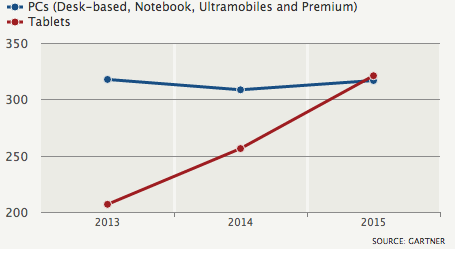
\includegraphics[width=0.50\textwidth]{tabletVsPC}
\caption{Worldwide Device Shipments (in millions) by Segment \cite{tabletOvertake}}
\label{fig:tabVsPC}
\end{figure}



\subsection{Android}\label{sec:Android}
The market share of the Android mobile operating system amongst mobile operating systems has been increasing steadily since 2012, going from 60\% in 2012 to 78\% in 2015 (see Figure~\ref{fig:android}), which helped influence the decision to develop the application for Android so as to have the widest possible reach.

\begin{figure}[h]
\centering
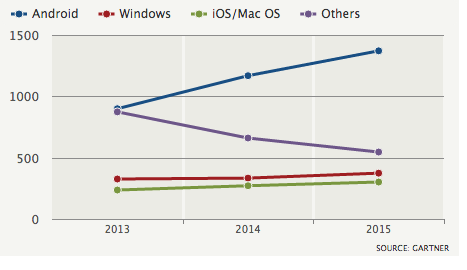
\includegraphics[width=0.50\textwidth]{android}\caption{Worldwide Device Shipments (in millions) by Operating System \cite{tabletOvertake}}
\label{fig:android}
\end{figure}


 

\subsection{M-learning}


CodeTouch falls into the self-paced E-Learning market, which is a market currently experiencing constant growth and is expected to do so for the foreseeable future. Today it is worth £31.1 billion and is growing with a compound annual interest rate of 7.6\%.
Things get even more encouraging when examining the m-Education market, defined as any form of e-Learning delivered to a mobile device, which is currently worth £6.1 billion worldwide .The market has a projected compound annual interest rate of 20.65\% from 2013-2018 10, meaning in 2019 the sector is predicted to be worth £12.93 billion.


\section{Target Audience}
CodeTouch is aimed at three main different types of users:
\begin{enumerate}
\item Beginner programmers who want to learn how to code
\item Pupils in schools studying Computing, especially at the Key Stage 3 level
\item Tablet owning developers who want to program on their devices
\end{enumerate}

\section{Existing Applications }
While I believe CodeTouch's interface to be unique in it's feel, approach and ease of use, there are existing applications with similar target audiences and objectives whose strengths and weaknesses I carefully studied when making functionality and design decisions throughout the duration of this project. 


\subsection{Scratch}\label{ssec:Scratch}
Scratch is perhaps the most successful "drag and drop" code-block based visual programming language, with over 7 million registered users \cite{scratchWebsite}. A free, open source project from the Lifelong Kindergarten Group at the MIT Media Lab, it has been very popular in educational establishments.

\begin{figure}[h]
\centering
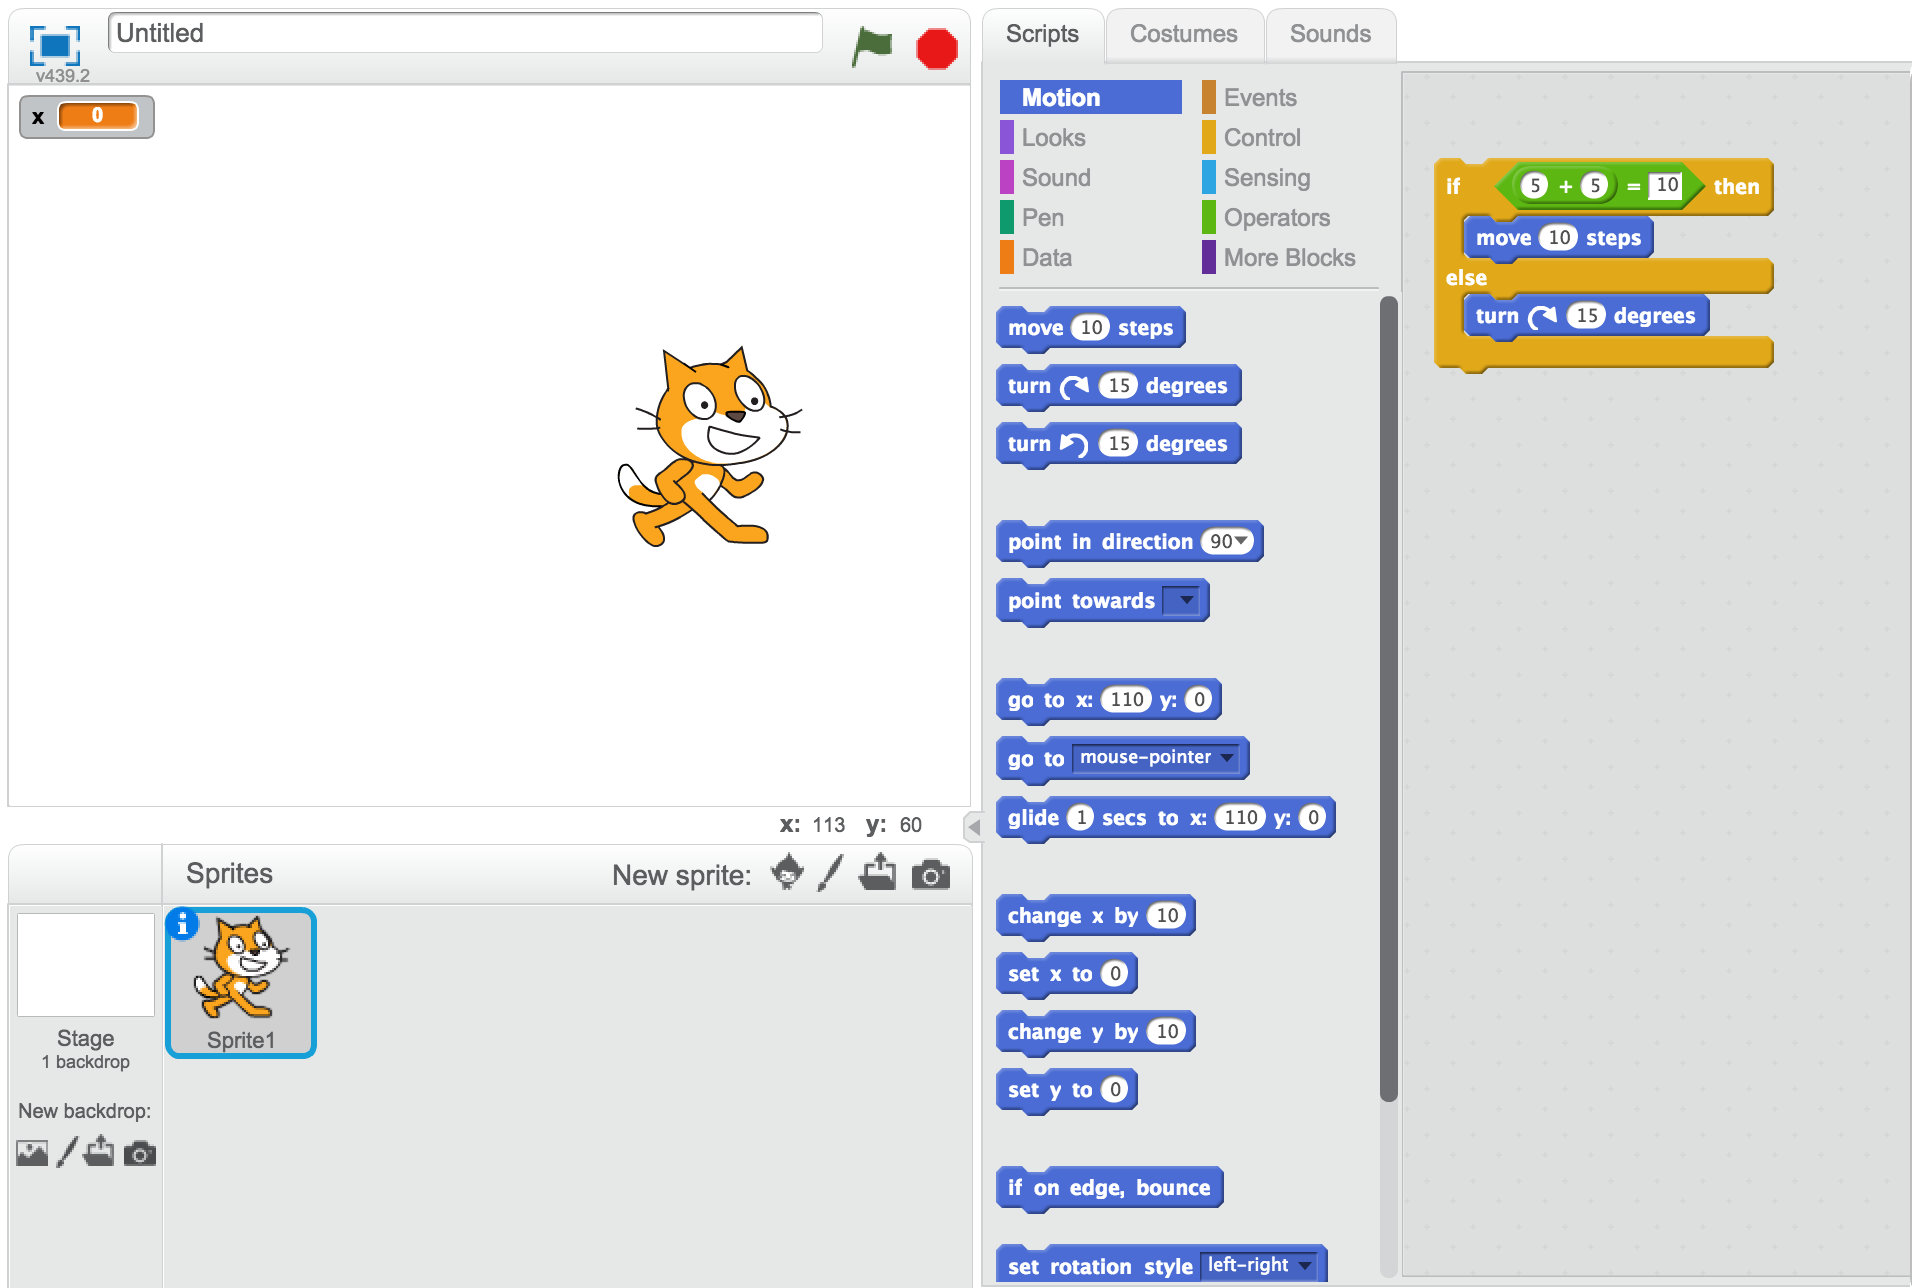
\includegraphics[width=0.9\textwidth]{scratch}
\caption{Scratch's Graphical User Interface}
\label{fig:scratchh}
\end{figure}

As is clear from its interface, shown Figure~\ref{fig:scratchh}, Scratch is squarely aimed at a younger audience. The user controls what it calls "Sprites" (for example the cat in Figure~\ref{fig:scratchh}) by dragging blocks of code from a menu onto a platform, where the shape of the blocks shows the user what blocks can work together. This approach is great in the sense that it is very clear what is and isn't valid, so the user doesn't have to worry about making syntax mistakes, they just have to make the shapes match. 

\subsection{CodeAcademy}\label{ssec:CodeAcademy}
CodeAcademy is an popular typing based tool that teaches programming through interactive lessons. Users are taught through step-by-step challenges and are rewarded with badges and experience points upon completion, encouraging users to return to the website. It contains tutorials for a host of languages, from web languages such as HTML and CSS to scripting languages like JavaScript and Python. 


\begin{figure}[h]
\centering
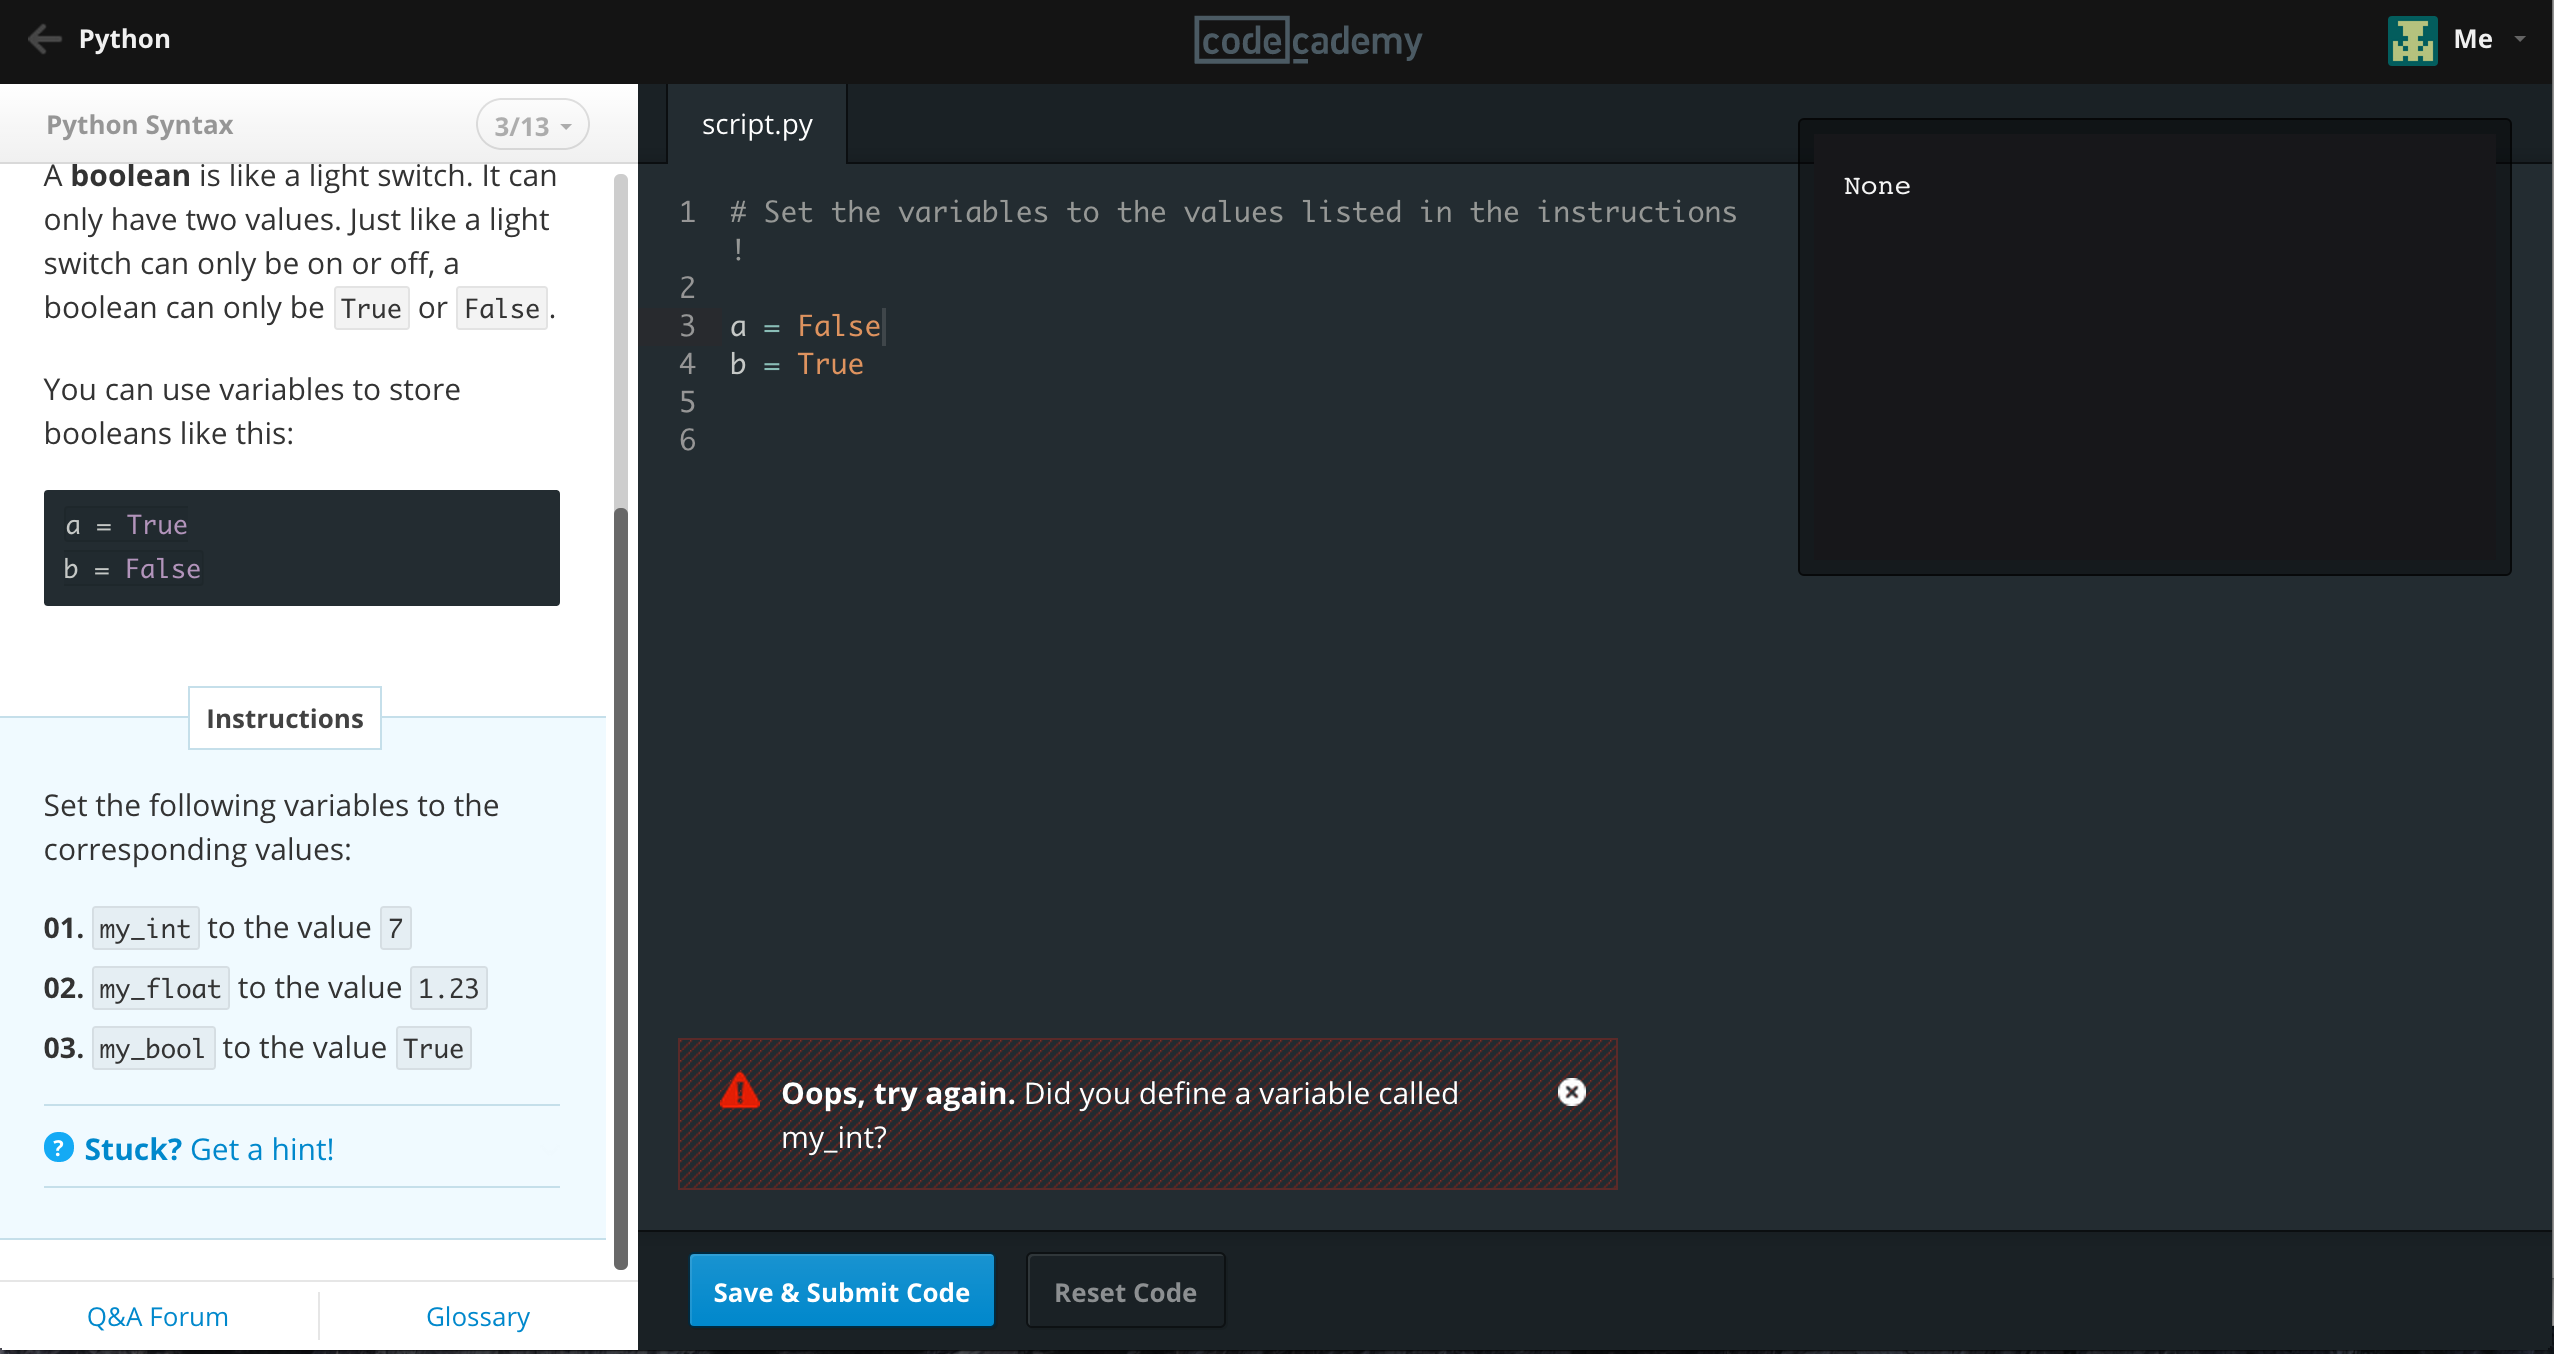
\includegraphics[width=0.9\textwidth]{CodeAcademy}
\caption{CodeAcademy's Graphical User Interface}
\label{fig:codeac}
\end{figure}

As shown in Figure~\ref{fig:codeac}, it has useful intelligent error reporting system that suggests where user may have gone wrong. CodeAcademy can be seen as a direct competitor to CodeTouch as has collaborated with the Department of Education to produce lessons for the new National Curriculum \ref{codeAcCu}, which have so far been taken up by over 1000 schools in the UK \ref{codeAcBr}. As part of this collaboration, a classroom management tool for schools has been made available to track pupils progress.




\subsection{TouchDevelop}{ssec:TD}
TouchDevelop is probably the most similar product that exists to CodeTouch. Developed by Microsoft, it is unique amongst CodeTouch's competitors in that it too takes input via button presses to produce textual code. Like CodeAcademy, it has step-by-step tutorials and has designed courses to fit the UK national curriculum. 

\begin{figure}[h]
\centering
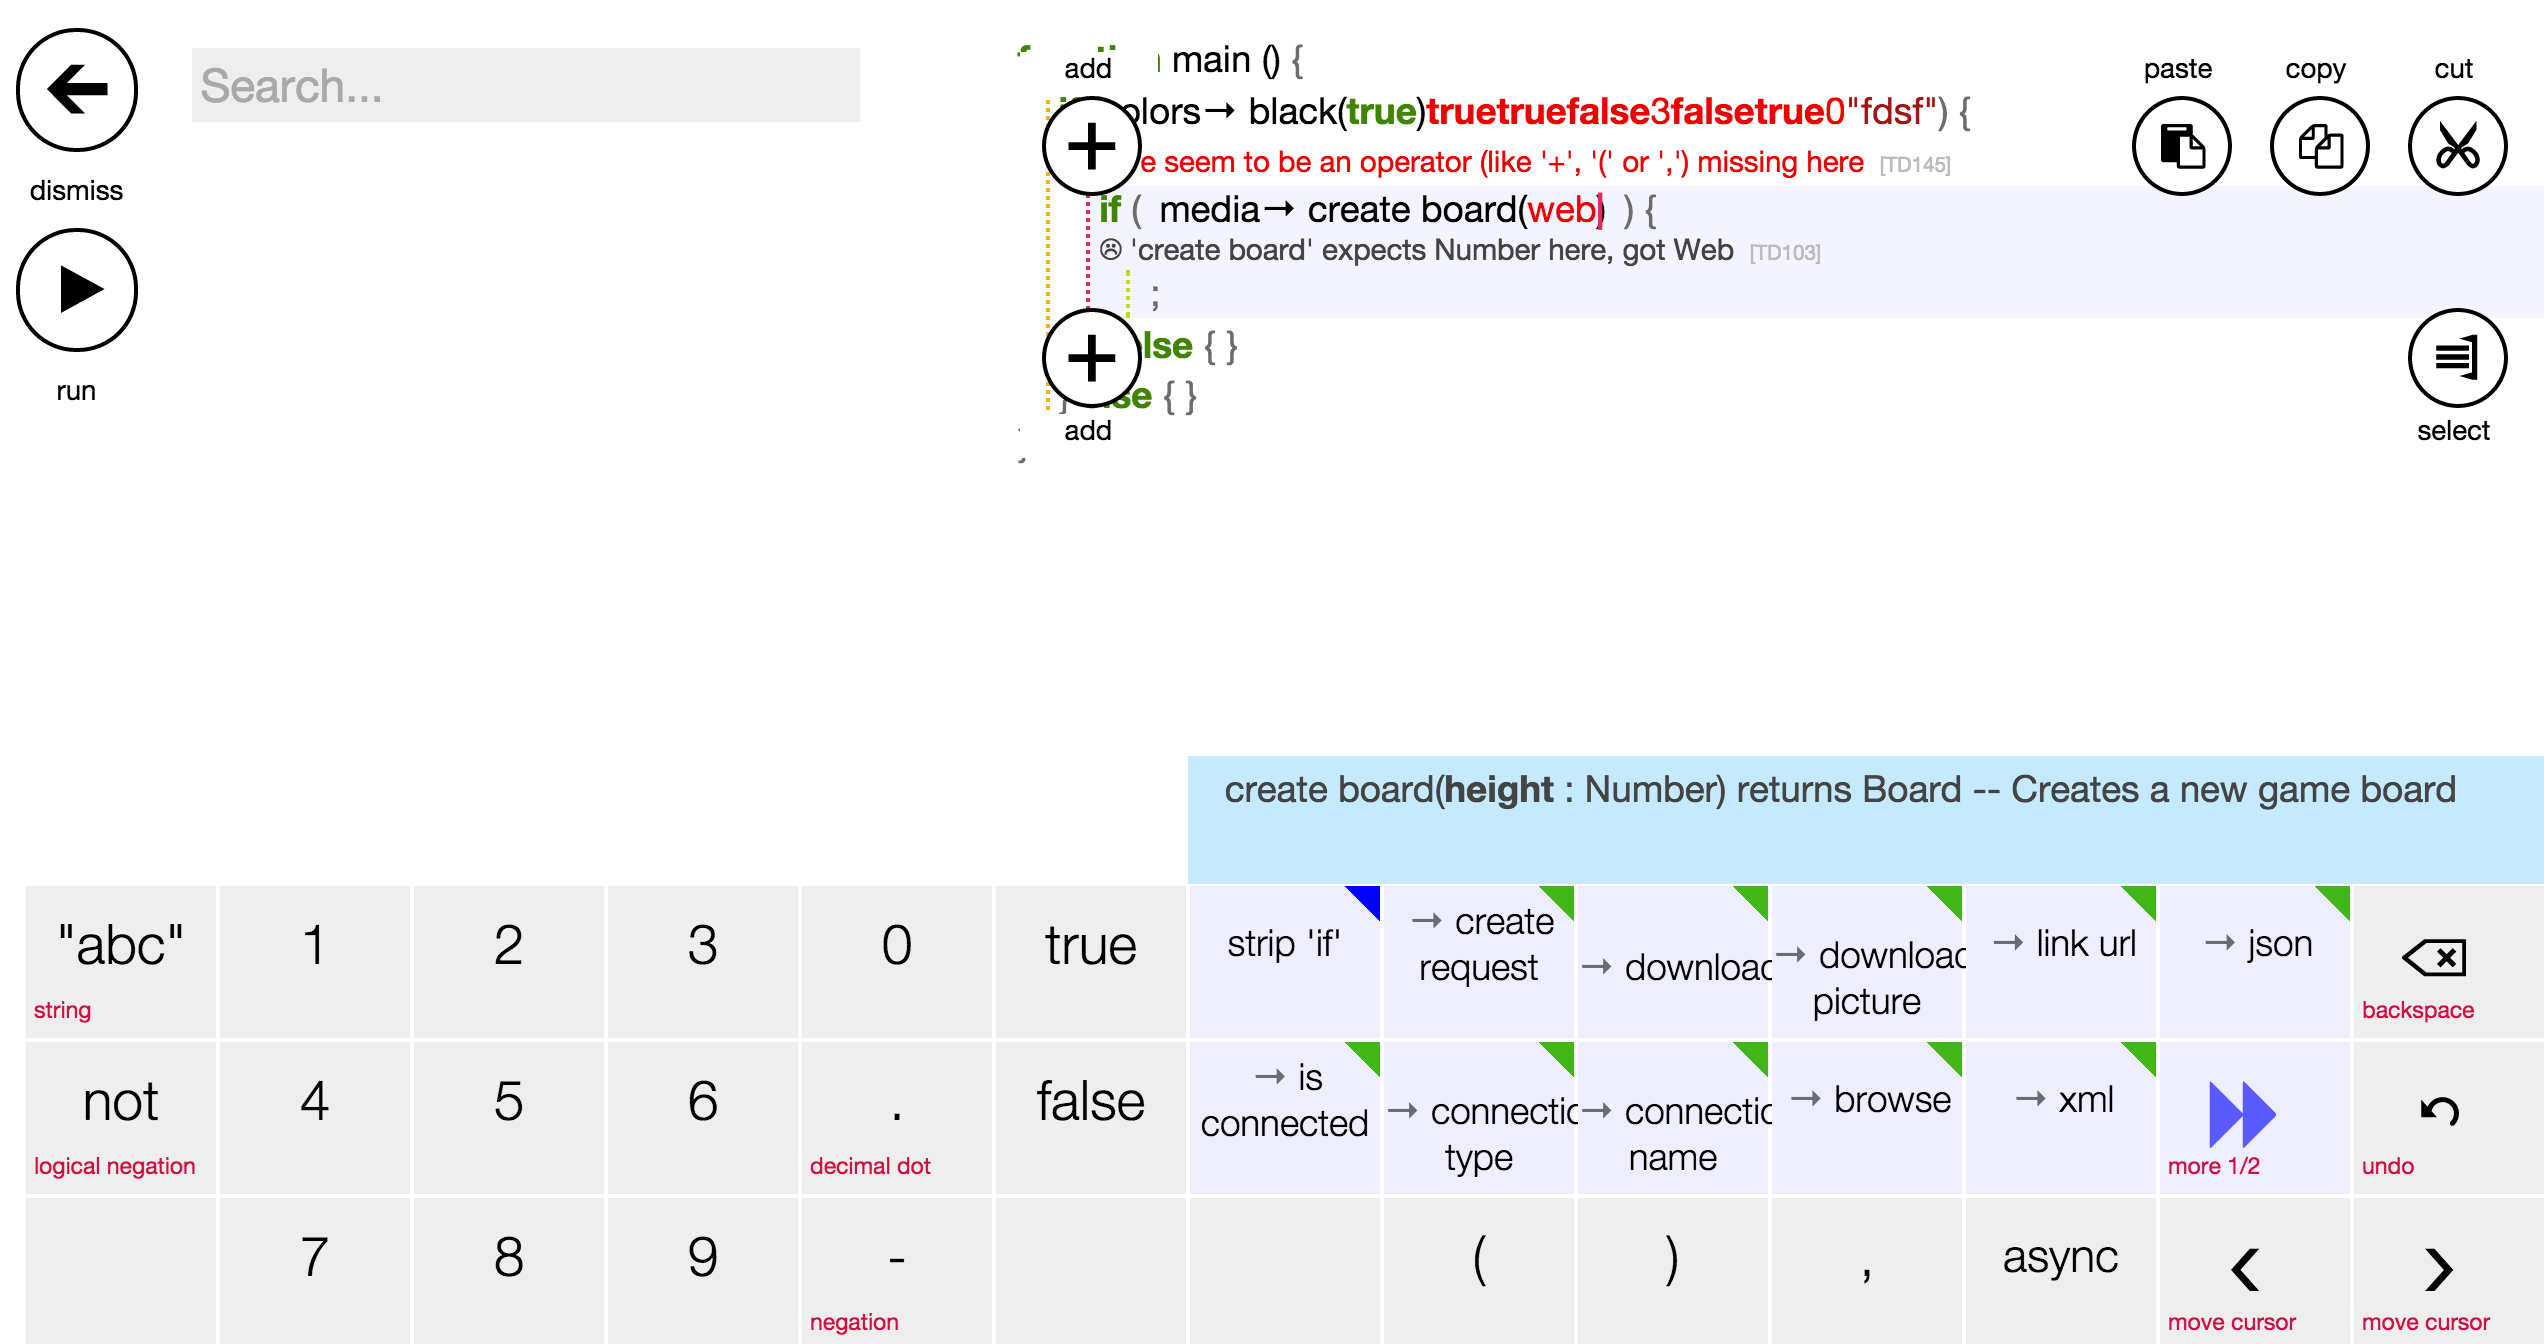
\includegraphics[width=0.9\textwidth]{touchdevelop}
\caption{TouchDevelops's Graphical User Interface}
\label{fig:touch}
\end{figure}

Although TouchDevelop has similar objectives to CodeTouch, there are some key differences in implentation and user experience. TouchDevelop has a large, complicated interface with a multitude of buttons on screen at any time (see Figure~\ref{fig:touch}), which slows down the coding process and gives it a clunky feel. Coding on TouchDevelop does not have the same flow as typing and feels unnatural, for example to declare a variable the user has to click where they want to declare it in the code, use the menu to choose the name then click on the code again after the assignment symbol. The same goes for adding functions and other programming paradigms such as \textbf{if} then \textbf{else} statements, all of which disrupts the flow of coding. TouchDevelop also allows the user to create syntactically incorrect code. 

TouchDevelop does not prevent the user from making syntax or semantic mistakes, as shown in Figure~\ref{fig:touch}, but it does provide suggestions for how to fix incorrect code. 





\section {Motivation and Objectives}
This shift towards tablets from computers \ref{ssec:shift}, combined with the upturn of people interested in learning how to code \ref{ssec:learnCode}, creates a very attractive opportunity for CodeTouch to take advantage of. As people start to use tablets for more of the things they would usually use a computer for, a programming app specifically aimed at the platform has the potential to be very popular. Moreover, the introduction of Computing to the UK National Curriculum, specifically the requirement to learn a textual language by Key Stage 3, has created a gap between the required and actual aptitude of school teachers who are struggling to implement the new policy with limited resources. By creating an application that makes teaching code easier for both teacher and pupil to learn, understand and produce real textual code, with the ease of the drag and drop code applications that pupils will be used to coming into Key Stage 3, CodeTouch has the capacity to be a powerful educational tool. 




In summary, the reasons for developing CodeTouch as are follows:

\begin{enumerate}
\item Help teachers to bridge the gap between visual code-block based coding and textual coding, a requirement of the new Key Stage 3 National Curriculum for Computing
\item Capitalise on coding's recent burst of popularity by designing an easy to use, intutive development environment for beginner programmers to learn the basics of programming.
\item Exploit the recent rise of the tablets to ubiquitous status by creating a coding environment designed for such devices, taking advantage of their touchscreen capabilities. 
\end{enumerate}

In order to achieve these goals, CodeTouch aims to create an integrated IDE with a unqiue interface and method of writing code that fits the following criteria:



\begin{enumerate}
\item Makes the most of the available space on a tablet screen
\item Exploits the benefits that a touch screen has over a conventional keyboard, most importantly it's dynamic nature
\item Creates a programming environment that removes the need to worry about syntax errors or semantic errors so that beginners can focus on learning the principles of writing code
\item Is as easy to use as visual code-block programming applications but produces textual output
\item Retains the free flowing feel of typing code on a keyboard
\item Helps teachers bring pupils understanding of computing to the required level as required by the sections of the Key Stage 3 National Curriculum articulated earlier in this document (see \ref{ssec:KS3})
\item Is fast and usable enough that it is also attractive to experienced coders as well as beginners
\end{enumerate}




% -----------------------------------------------------------------------------

\chapter{Technical Background}
\label{chap:technical}


Before development could begin there were a number of decisions that had to be made regarding the technology options available, and which ones would be most suited for CodeTouch in order to best achieve the projects goals. Here I will outline the different options and explain their strengths and weaknesses. 

\section{Different Type Of Mobile Application }\label{sec:ApTypes}
At time of writing, there are 3 main types of mobile application:
\begin{enumerate}
\item \textbf{Native Application}
\begin{itemize}
\item A Native Application is written in a specific programming language for a specific hardware platform, for example Java for Android with Android, Objective C with iOS and C# for Windows Phone. Native apps are the best option in terms of performance as they can access the hardware of the device it is running on. Debugging is also easier, however the single platform nature of native applications make them more expensive to develop and maintain if cross platform coverage is desired, as companies need to do everything multiple times and potentially employ experts in multiple programming languages in order to maintain their app. 
\end{itemize}


\item \textbf{Cross-Platform Application}
\begin{itemize}
\item A Cross-Platform Application is an application written in a generic web language, most commonly HTML5, in order to be runnable on all mobile applications, which is an obvious advantage over developing nativley.  Other advantages include being able to update the application centrally, removing the need for the user to download updates.  However, having to accommodate for all different types of browser can cause maintenance problems, and the fact that Cross-Platform apps cannot be uploaded to the native Application stores (such as Apple's App Store and Google's Play Store) may put off potential users as the apps security cannot be verified. Furthermore, they do not perform as quickly as native apps and due to their cross-platform nature, have to look the same on all devices, which can make them look unnatural. 
\end{itemize}
\item \textbf {Hybrid Application}
\begin{itemize}
\item A Hybrid Application aims to  combine the advantages of native and web app development. They are developed in generic web languages but are wrapped in native code. This means they can be cross platform but still take advantage of the devices in-built features. However, they still retain the disadvantages of cross-platform apps in that they do not perform as well and can look unnatural.
\end{itemize}
\end{enumerate}



\section{Android}
\subsection{Overview}
CodeTouch is developed for Android devices. Although Android is now a household name, I will briefly describe it's key features. Android is an Operating System (OS) for mobile devices, developed by Google. It is the most popular mobile OS in the world, thanks in part to Google making it open source, allowing third party smartphone and tablet manufacturers to use it as the OS for their devices. 

\subsection{Language}
Android's native language is Java for Android, a language very similar to Java. There are barely any noticeable differences between the two languages for the developer , it's main differences are in how it is compiled. Normal Java compiles code into Java bytecode and runs it on a Java Virtual Machine (an abstract computing machine which allows a computer to run a Java program). Android for Java instead compiles code into a specialised bytecode format and run's in on a purposely designed virtual machine called Davlik, which was designed to use less space than Java Virtual Machine, for obvious reasons given mobile devices limited memory capacities. 

\subsection{Layout}
There are two ways of programming the layouts for Android applications, either defining it programatically in the main application source code or writing it in XML in a separate layout file. For a multitude of reasons, it is common convention to write most of it out in XML. One advantage is that as it is separate from the main source code, it can be modified without having to change and recompile the application. This makes creating and testing different layout options much easier than having to edit the source code. As it is all in one document it also makes visualising the UI's structure easier. 


There are also benefits of declaring layout elements in the source code, for example being able to dynamically create layout elements and being able to define many layout elements at once using loops.

For CodeTouch, the main structure of the layout is defined in XML, with some additional elements being defined in the source code, such as the variable buttons that needed to be created dynamically. 




\subsection{Android Integrated Development Environments (IDE)}\label{sec:andIDE}
An Integrate Development Environment, in the case of mobile applications, is an application that allows the editing, compiling, debugging, GUI building and running of mobile application source code. There are a range of different options for choosing an IDE for Android Development, but when CodeTouch development started there were two conventional options: Eclipse and Android Studio, Google's own IDE. 
\begin{enumerate}
\item Eclipse
\begin{itemize}
\item Pros
\begin{itemize}
\item Currently compiles faster than Android Studio.
\end{itemize}
\end{itemize}
\begin{itemize}
\item Cons
\begin{itemize}
\item Eclipse Android plugin no longer being developed (Announced June 2015)
\end{itemize}
\end{itemize}

\item Android Studio
\begin{itemize}
\item Pros
\begin{itemize}
\item Better support as is developed by Google
\item Improved auto-completion options over Eclipse
\end{itemize}
\end{itemize}
\begin{itemize}
\item Cons
\begin{itemize}
\item Compilation can be very slow, sometimes taking minutes at a time.
\end{itemize}
\end{itemize}
\end{enumerate}





\subsection{Android Device Monitor}
Android Device Monitor is a program that accompanies Android Studio which provides a GUI for debugging Android apps. In particular it contains a tool called Traceview which can produce visual and textual information about what sections of code are being called most often and for how long, a tool which came in very useful when trying to locate bottlenecks in order to optimise the running of the program.

INCLUDE IMAGE OF TRACEVIEW

\section{Programming Languages}


\subsection{Overview}
At a high level, a programming language is a language constructed to relay instructions to a computer. More specifically, a language is usually described by two components, it's \textbf{syntax} and it's \textbf{semantics}.

\subsubsection{Syntax}
From Wikipedia:

\begin{quote}

\textit{The syntax of a computer language is the set of rules that defines the combinations of symbols that are considered to be a correctly structured document or fragment in that language.}
\end{quote}

In plainer terms, the syntax of a language refers to the rules that determine whether a program is structurally sound. This is easier to understand by comparing it to the syntax of the English language. A sentence is considered to be syntactically correct if all the words it contains are valid in the positions they are in. For example the sentence "He chair" is not syntactically correct as a noun cannot follow a pronoun.

The syntax of a language is traditionally made up of three sections:
\begin{itemize}
\item {Lexical Syntax: }
This is the set of all valid tokens in a language. A token can be thought of a single element of a language. To use the English language analogy again, a token would be like the set of all valid words and punctuation marks. 

\item{Concrete Syntax: }
The concrete syntax of a language is the set of rules that describe a language. In most languages, it can be expressed by a \textbf{Context Free Grammar (CFG)}. A CFG $G\,$ can be described by the 4 tuple\cite{Sipser}:

$G\,$ = ( $V\,$, $\Sigma$ , $R\,$, $S\,$ ) where:

\begin{itemize}
\item
$V\,$  is a finite set, whose elements are called variables
\item
$\Sigma$ is a finite set, whose elements are called terminals
\item $V\,$ $\cap$ $\Sigma$ = $\emptyset$,
\item
$R\,$ is a finite relation from V to ($V\,\cup\Sigma$)$^{*}\,$. The members of $R\,$ are called the rules or productions of the grammar. 
\item
$S\,$ is the start variable , used to represent the whole sentence (or program). It must be an element of $V\,$.
\end{itemize}



\item{Abstract Syntax: }
An optimised internal representation of the program which is defined by a simpler grammar. 
\end{itemize}


\subsubsection{Semantics}
While syntax refers to the structure of a language, semantics concerns it's meaning, or what it does. More formally: 

\begin{quote}
\textit{The semantics of a programming language describe the relationship between the syntax and the model of computation\cite{semantics}.}
\end{quote}

To demonstrate this let's look at an example: 

\begin{lstlisting}[language=Java]
int a = 0;
for( int i = 0; i < 10; i++){
    a = a + 1;
}
\end{lstlisting}

If we were to analyse this syntactically, all we could say about it is that it is a valid combination of symbols for the Java language. On the other hand, if we were to analyse it semantically we would say that this source code declares a new integer variable $a$ with an initial value of 0, then increments this value by 1 a total of 10 times, giving it a final value of 10. 

Another example that illustrates the difference between the syntactical and semantical properties of a code is the following two Java snippets:

\begin{figure}[h]
\centering
\begin{subfigure}{0.5\textwidth}
  \centering

\begin{lstlisting}[language=Java]
int a = 10;
if( a > 0 ){
    System.out.println("Hello world");
}else{
    System.out.println("Goodbye world");
}
\end{lstlisting}


\end{subfigure}%
\begin{subfigure}{0.5\textwidth}
  \centering
\begin{lstlisting}[language=Java]
//
int a = 10;
if( a > 0 ){
    System.out.println("Hello world");
}
//
\end{lstlisting}


\end{subfigure}
\label{fig:success}
\end{figure}

Syntactically, the two pieces of code are distinct, as the one on the left contains extra symbols. Semantically, however, they are exactly the same, as they both declare a new variable a and output= the text "hello word".





\section{Compilation}
The compilation process is the sequence of events that turns source code into a sequence of instructions that a computer an understand. This is necessary because most code is written in a high level language designed to be easily understood by humans rather than machines. It can be split into the following main sections \cite{compiler}:

\begin{center}

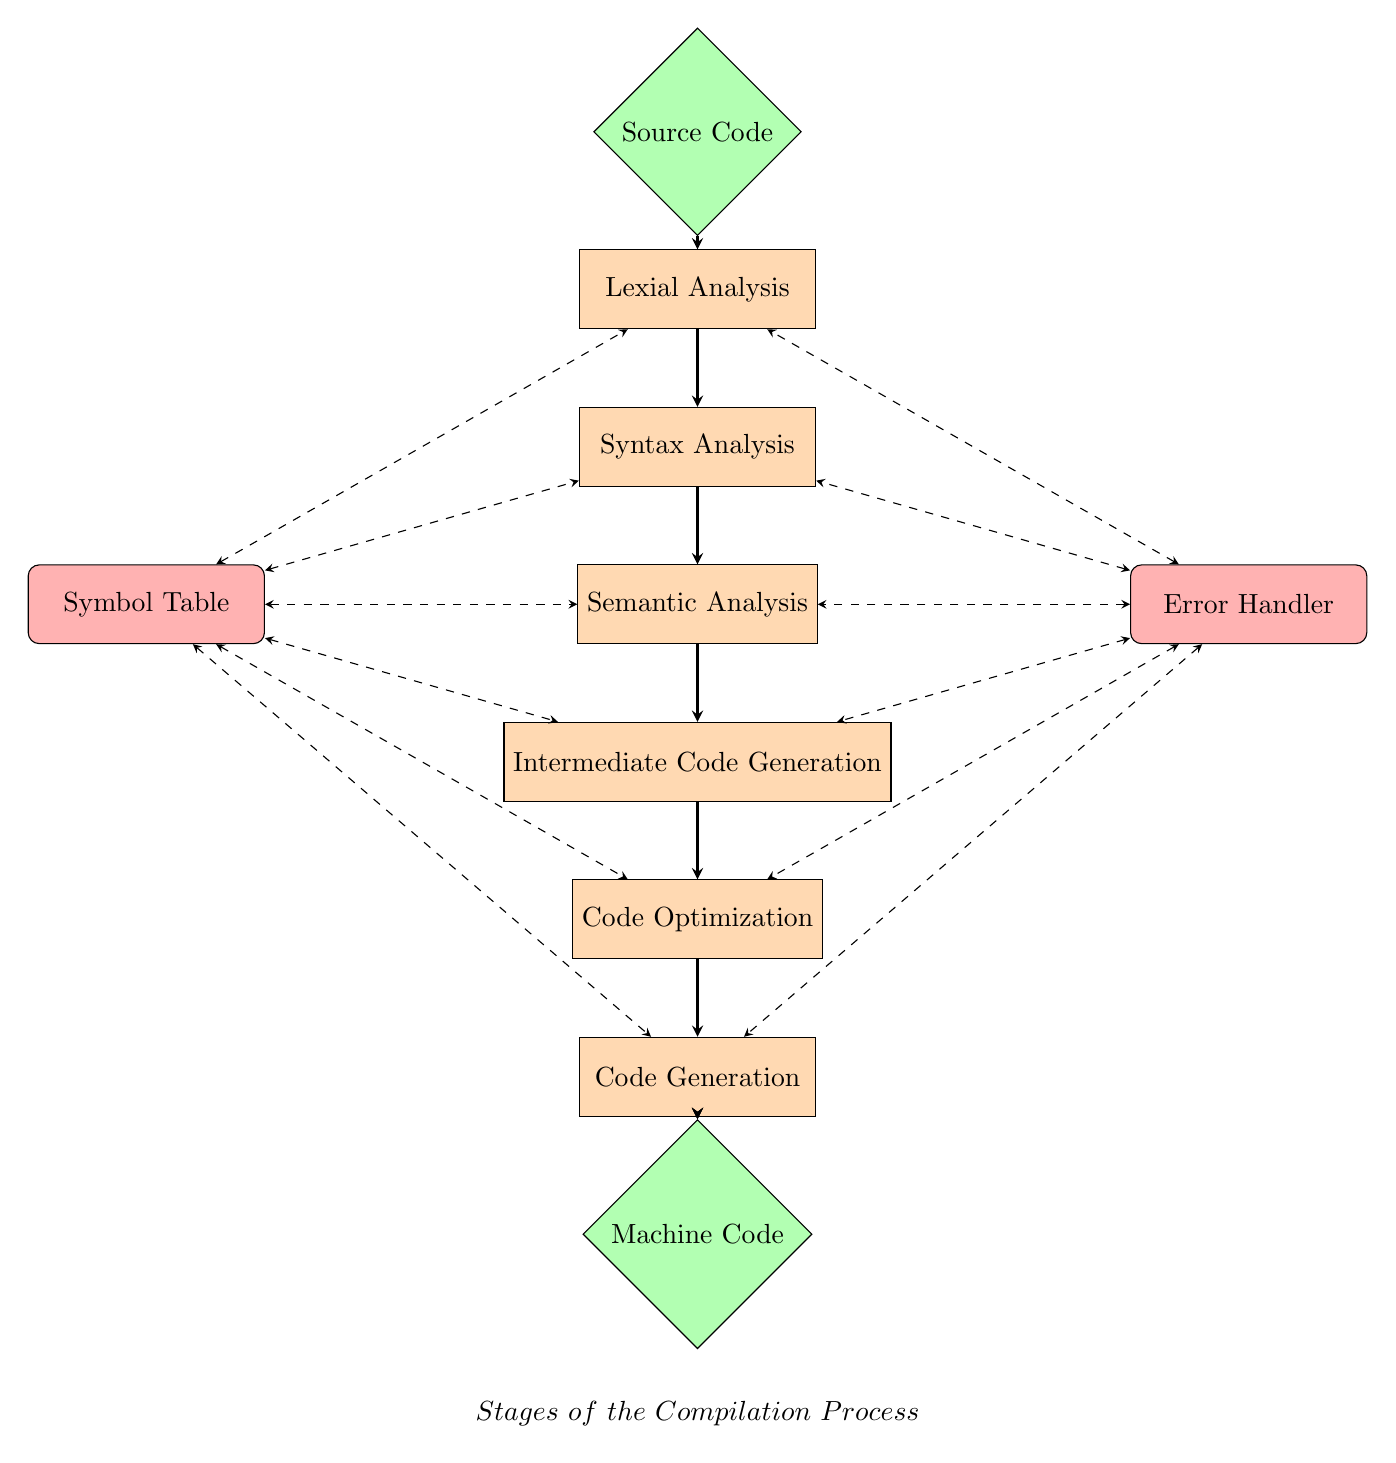
\begin{tikzpicture}[node distance=2cm]

\node (start) [decision] {Source Code};
\node (a1) [process, below of=start] {Lexial Analysis};
\node (a2) [process, below of=a1] {Syntax Analysis};
\node (a3) [process, below of=a2] {Semantic Analysis};
\node (a4) [process, below of=a3] {Intermediate Code Generation};
\node (r1) [startstop, right of=a3, xshift=5cm] {Error Handler};
\node (l1) [startstop, left of=a3, xshift=-5cm] {Symbol Table};

\node (a5) [process, below of=a4] {Code Optimization};
\node (a6) [process, below of=a5] {Code Generation};
\node (end) [decision, below of=a6] {Machine Code};
\draw [arrow, below of=a1] (a1) -- (a2);
\draw [arrow, below of=a1] (a2) -- (a3);
\draw [arrow, below of=a1] (a3) -- (a4);
\draw [arrow, below of=a1] (a4) -- (a5);
\draw [arrow, below of=a1] (a5) -- (a6);
\draw [arrow, below of=a1] (a6) -- (end);
\draw [arrow2] (l1) -- (a1);
\draw [arrow2] (l1) -- (a2);
\draw [arrow2] (l1) -- (a3);
\draw [arrow2] (l1) -- (a4);
\draw [arrow2] (l1) -- (a5);
\draw [arrow2] (l1) -- (a6);
\draw [arrow2] (r1) -- (a1);
\draw [arrow2] (r1) -- (a2);
\draw [arrow2] (r1) -- (a3);
\draw [arrow2] (r1) -- (a4);
\draw [arrow2] (r1) -- (a5);
\draw [arrow2] (r1) -- (a6);
\draw [arrow] (start) -- (a1);
\draw [arrow] (a6) -- (end);
\draw [arrow] (a6) -- (end);
\node [below=2cm, align=flush center,text width=10cm] at (end)
        {
           $Stages$ $of$ $the$ $Compilation$ $Process$
        };
\end{tikzpicture}


\end{center}

As is shown from the diagram, at each step of compilation errors can be detected and reported. Also important is the symbol table. This can have differing purposes depending on what language is being compiled:

\begin{itemize}
\item To store a reserve list keywords in a language that cannot be used for other purposes
\item To store variable names and their scope
\item To implement type checking
\item To store information about variable scope

\subsection{Lexical Analysis}

\begin{itemize}
\item[]
In traditional programming languages, the is the process of converting an input stream of characters (the code) into tokens (tokenization). This step will determine whether the code it has been given is indeed made up of valid tokens. This process has several sub processes. It will remove and white spaces and comments, split the input stream into what are known as lexeme (a lexical unit of a language that is made up of one of several characters, which do not make sense separately), then pass these lexeme to a series of recognisers that will categorise them into tokens. These could include recognisers such as:

\begin{enumerate}
\item A keyword recogniser, categorises keyword tokens by consulting a list of keywords that cannot be used as identifiers (for example \textbf{null} or {String} in Java). 
\item An identifier recogniser, which categorises identifier token such as variables. 
\item A numerical constant recogniser, which categorises numerical tokens
\item An string constant recogniser, which categorises string tokens
\item An operator recogniser, which categorises operator tokens
\item A recogniser to categorise other tokens that contribute to the structure  of the code, such as semi-colons and parenthesis.
\end{enumerate}


For some tokens, additional information is stored, for example a variable would store the name of the variable as well. 

There are many ways of doing lexical analysis, but to illustrate the point clearly I will now demonstrate an example of lexical analysis:








\begin{table}[!h]
\begin{center}
    \begin{tabular}{ |  l |   l | }
    \hline
    \textbf{Lexeme} & \textbf{Token}\\ \hline
    a & a\\ \hline
    = & = \\ \hline
    b & ID(b)  \\ \hline
    - & - \\ \hline
    c & ID(c) \\ \hline
    *  & * \\ \hline
    d & ID(c)  \\ \hline

    \end{tabular}
        \caption {Possibe lexical analysis of code}
\label{name}
\end{center}
\end{table}




\end{itemize}

The example above shows an example tokenization of the given code, where ID(a) means a keyword token with value a.

At this stage, there are very few errors that can be detected. At most, it can invalid tokens (for example, an illegal symbol). 








\subsection{Syntactic Analysis}\label{ssec:contextfreelanguage}



This step takes the tokens generated from Lexical analysis and determines if they fit the grammar of a language by attempting to create a parse tree from the tokens, using the language's Context Free Grammar. We call the parse tree generated a Concrete Syntax Tree. 
\item []

For example, we can define the language $G\,$ as follows:

$G\,$ = 
(\big\{ $\langle$ EXP $\rangle$, $\langle$ ID$\rangle$, $\langle$ ASSIGN$\rangle$ \big\}, \big\{$ a, b, c, d, +, -, = $\big\}, $R\,$, $\big\{\langle$ ASSIGN $\rangle$ \big\} ) 

The rules of the grammar are often expressed in Backus-Naur Form (BNF):
\newline



$R\,$ $=\,$ 
$\langle ASSIGN \rangle$ $\rightarrow$ $\langle EXP \rangle$ = $\langle EXP \rangle$

$\langle EXP \rangle$ $\rightarrow$  $\langle ID \rangle$ + $\langle EXP \rangle$  $|$  $\langle ID \rangle$ - $\langle EXP \rangle$ $|$ $\langle ID \rangle$ 



$\langle ID \rangle$ $\rightarrow$ $a | b | c | d$


At this stage, structural errors in the code can be detected. 
Broadly speaking, there are two approaches to parsing, top down and bottom up. Top-down parsing starts with the start symbol of the grammar and uses the rules to try and get to the given statement. If it can successfully, it is declared syntactically correct. 

Bottom-up parsing starts with the statement and works up the rules to try and get to the start symbol. 

The other factor that must be considered when parsing is whether to use a leftmost derivation parser or a rightmost derivation parser. A leftmost derivation parser moves through the tree evaluating all non-terminal statements on the left first, and a rightmost derivation parser does the same but with the right. 

It is not necessary for the scope of this project to understand the nuances of leftmost and rightmost derivation parsers, nor the differences between top-down and bottom-up parsing. In order to illustrate how parsing works I will now present an example of a leftmost derivation, top-down parser, as this is the easiest to comprehend and adequately demonstrates the process of parsing. 



\begin{figure}[h]
\centering
\begin{subfigure}{0.7\textwidth}
  \centering

\Tree[.$\langle$ASSIGN$\rangle$ [.$\langle$EXP$\rangle$ [.$\langle$ID$\rangle$ [.a ] ]]
            [.$=$ ]
          [.$\langle$EXP$\rangle$ [.$\langle$ID$\rangle$ [.b ]]
            [.$-$ ]
                [.$\langle$EXP$\rangle$ [.$\langle$ID$\rangle$ [.c ]]
            [.$*$ ]
                [.$\langle$EXP$\rangle$ [.$\langle$ID$\rangle$ [.d
]]]]]]


\end{subfigure}%
\begin{subfigure}{0.7\textwidth}
  \centering
        \begin{enumerate}
          \item $\langle ASSIGN \rangle    $\\      
            \item $\langle EXP \rangle = \langle EXP \rangle $\\
            \item $\langle ID \rangle = \langle EXP \rangle$ \\
            \item $a = \langle EXP \rangle $\\
            \item $a = \langle ID \rangle - \langle EXP \rangle $\\
            \item $a = b - \langle EXP \rangle $\\
            \item $a = b - \langle ID \rangle * \langle EXP \rangle $\\
            \item $a = b - c * \langle EXP \rangle $\\
            \item $a = b - c * \langle ID \rangle $\\
            \item $a = b - c * d $\\
        \end{enumerate}

\end{subfigure}
\caption{$a = b - c * d$}
\label{fig:success}
\end{figure}

Figure~\ref{fig:success} shows a successful top down, leftmost derivation parsing of the code $a = b - c * d$ using grammar $G$. The left hand side of the diagram shows the resulting parse tree and the right hand side shows the derivation steps. As you can see in step 1, we start with the start symbol of the grammar, $\langle ASSIGN \rangle$. If we recall the first rule from $R$:

\begin{center}
$\langle ASSIGN \rangle$ $\rightarrow$ $\langle EXP \rangle$ = $\langle EXP \rangle$
\end{center}
we can see that our code, $a = b - c * d$, can fit this as we can put $a$ into the left side and $b - c * d$ into the right side, giving us
$\langle EXP \rangle$ = $\langle EXP \rangle$.

From here, as we are evaluating the left hand side first, the parser now looks for the left most non-terminal symbol, which in this case is $\langle EXP \rangle$, which contains only $a$. 

If we recall the second rule from $R$:
\begin{center}
$\langle EXP \rangle$ $\rightarrow$  $\langle ID \rangle$ + $\langle EXP \rangle$  $|$  $\langle ID \rangle$ - $\langle EXP \rangle$ $|$ $\langle ID \rangle$ 
\end{center}

we can see that $a$ will not fit into either of the first two conditions, $\langle ID \rangle$ + $\langle EXP \rangle$  or  $\langle ID \rangle$ - $\langle EXP \rangle$, but it will fit into $\langle ID \rangle$, so $\langle EXP \rangle$  evaluates to $\langle ID \rangle$, leaving us with the derviation $\langle ID \rangle$ = $\langle EXP \rangle$ to evaluate.

Now the left most non-terminal symbol is $\langle ID \rangle$, which we can evaluate using the third rule of $R$:

\begin{center}
$\langle ID \rangle$ $\rightarrow$ $a | b | c | d$
\end{center}

resulting in the derviation $\langle ID \rangle$ = $\langle EXP \rangle$.. 

The parser carries on in this fashion until it there are no more non-terminal symbols left, in this instance after a total of 10 derivation steps, and declares the statement syntactically correct. 
I will now show an example of a statement that does not fit the grammar. 




\begin{figure}[h]
\centering
\begin{subfigure}{.5\textwidth}
  \centering
  
  \Tree[.$\langle$ASSIGN$\rangle$ [.$\langle$EXP$\rangle$ [.$\langle$ID$\rangle$ [.a ] ]]
            [.$=$ ]
          [.$\langle$EXP$\rangle$ [.$?\,?\,?\,$ ]]
]

\end{subfigure}%
\begin{subfigure}{.5\textwidth}
  \centering
  \begin{enumerate}
  \item $\langle ASSIGN \rangle    $\\      
\item $\langle EXP \rangle = \langle EXP \rangle $\\
\item $\langle ID \rangle = \langle EXP \rangle$ \\
\item $a = \langle EXP \rangle $\\
\item $a$ = $???$ \\
\end{enumerate}

\end{subfigure}
\caption{$a$ = $b$ $c$}
\label{fig:test}
\end{figure}

In this example, we try and parse the code $a$ = $b$ $c$. The first 4 steps are the same as the the example from Figure~\ref{fig:success}, but then we run into a problem. The leftmost non-terminal symbol,  $\langle EXP \rangle $, contains $b$ then $c$. From the second rule of R:

\begin{center}
$\langle EXP \rangle$ $\rightarrow$  $\langle ID \rangle$ + $\langle EXP \rangle$  $|$  $\langle ID \rangle$ - $\langle EXP \rangle$ $|$ $\langle ID \rangle$ 
\end{center}

we can see that $\langle EXP \rangle$ has to either evaluate to something + something, something - something or something by itself. The statement $b$ $c$ cannot fit into any of these categories, so the parser declares the code not syntactically correct. 


\end{itemize}


\subsection{Ambiguous Grammars}
Before we move on, it is important to note that when building a grammar to build a Concrete Syntax Tree, a highly desirable property is that of \textbf{unambiguity}. To say a grammar is ambiguous is to say that one string can have more than one distinct valid parse trees. The problem with this is that these parse trees, although all having the same value syntactically, can have completely different meanings semantically. 

For example, to perform mathematical operations, it is intuitive to define the grammar $G1$ as:
\\
$G1\,$ = \begin{centering} 
(\big\{ $\langle$ EXP $\rangle$, $\langle$ NUM$\rangle$, \big\}, \big\{$a,b, c, +, -, *, /, \wedge $\big\}, $R\,$, $\big\{\langle$ EXP $\rangle$ \big\} ) \end{centering}
\\
\\
$R\,$ $=\,$ 
$\langle EXP \rangle$ $\rightarrow$ \begin{centering}$\langle EXP \rangle$ + $\langle EXP \rangle$  $|$ \\ $\langle EXP \rangle$ - $\langle EXP \rangle$ $|$ \\ $\langle EXP \rangle$ * $\langle EXP \rangle$ $|$ \\ $\langle EXP \rangle$ / $\langle EXP \rangle$ $|$ \\ $\langle EXP \rangle$ \wedge $\langle EXP \rangle$ $|$ \\ $a$ $|$  $b$ $|$  $c$ \\ \end{centering}
\\
\\
\linebreak
However, this is unambiguous as it can produce different trees with different meanings depending on the parser. 




\begin{figure}[h]
\centering
\begin{subfigure}{.5\textwidth}
  \centering
\Tree[.$\langle$EXP$\rangle$ [.$\langle$EXP$\rangle$ [.$\langle$EXP$\rangle$ [.a ] ]
            [.$+$ ]
                [.$\langle$EXP$\rangle$ [.c ]
]]
            [.$*$ ]
          [.$\langle$EXP$\rangle$ [.a ]]]
          \caption{}\label{fig:left}
\end{subfigure}%
\begin{subfigure}{.5\textwidth}
  \centering
\Tree[.$\langle$EXP$\rangle$ [.$\langle$EXP$\rangle$ [.a ]]
            [.$+$ ]
          [.$\langle$EXP$\rangle$ [.$\langle$EXP$\rangle$ [.b ] ]
            [.$*$ ]
                [.$\langle$EXP$\rangle$ [.c ]
]]]
\caption{}\label{fig:right}
\end{subfigure}%
\caption{Leftmost derivative (a) and rightmost derivative parse trees for $a + b * c$}\label{fig:both}
\end{figure}

The two trees in Figure~\ref{fig:both} are both valid parse trees for $a + b * c$, but Figure~\ref{fig:left} has the semantic meaning of (a+b)*c while Figure~\ref{fig:right} has the semantic meaning of a+(b*c). 

There are some cases where ambiguity is unavoidable in a language, such as in C++:

\begin{lstlisting}[language=Java]
    x * y ;
\end{lstlisting}

This can mean two different things depending on what has happened so far in the program:
\begin{enumerate}

\item The declaration of y, as pointer to type x
\item The multiplication of x and y, throwing away the answer.

\end{enumerate}

This distinction is not possible with a Context-Free Grammar, so most C++ compilers will combine the parsing with a lookup table, meaning  that once it sees, the parser knows whether x has been defined to a type or not. However, this means it is not a Context-Free Grammar as it is relying on context. We say this is now a \textbf{Context-Sensative Grammar (CSG)}. It is also worth noting that using CFGs and CSGs are not the only two option available, there exists a host of alternative parsing options, but they are less common and it would be beyond the scope of this document to present and explain every distinct method of parsing that has ever been invented. 



\subsection{Semantical Analysis}
This stage analyses whether the source code provided makes sense or not. The main tasks involved in this are:
\begin{itemize}
\item \textbf{Scope Resolution} \\ This is the process of checking whether a variable that has been called is accessible from the position in the code it is in. To use a Java snippet as an example:
\begin{lstlisting}[language=Java]
    if(true){
        int a;
    }
    a = 5;
\end{lstlisting}
This code would pass syntactical analysis, as all the symbols are valid tokens and are arranged in a structurally correct manner, however semantic analysis of this code should report an error because on the line $a = 5$, the variable $a$ is not in scope. This is because it has been declared inside an if statement.
\\
\item \textbf{Type Checking} \\ This is the process of determine whether a statement uses variable types correctly. To use another Java snippet as an example:
\begin{lstlisting}[language=Java]
    Boolean b = 3;
    int i = "foo";
    String a = b && i;
\end{lstlisting}

This code would again probably pass sytactial analysis (depending on the sophistication of the analysis), but there are multiple type errors here that mean it doesn't make sense semantically. For example, the Boolean $b$ is being declared with a numerical value, the int $i$ is being declared with a String value and on the third line a Boolean operation is being performed on a Boolean and an int.
\\
\item \textbf{Array-bound checking} \\ This is the process of ensuring that any array index calls are within the limits of that array. The following C++ code illustrates an array-bound checking error:
\begin{lstlisting}[language=Java]
    double exampleArray [ 6 ];
    exampleArray[7] = 4;
    
\end{lstlisting}

This code declares an array of doubles, with the parameter 6, indicating that indexes 0-5 are valid. The next line tries to call $exampleArray$ with an index of 7, which is out of range. At this stage, an error should be reported.  


\end{itemize}


\subsection{Intermediate Code Generation}\label{ssec:icm}
The parse tree generated from the syntactical analysis can be said to be a Concrete Syntax Tree, in that it exactly represents the source code. This often contains many nodes which are unessential for understanding the actions of the code, such as parentheses and semi-colons. The next step it to optimise this tree as much as possible for the later stages of the compiler. This is done by creating what is known as an
\textbf{Abstract Syntax Tree (AST)} from the Concrete Syntax Tree. 


\begin{figure}[!h]
\centering
\begin{subfigure}{.5\textwidth}
  \centering
  
\Tree[.$\langle$ASSIGN$\rangle$ [.$\langle$EXP$\rangle$ [.$\langle$ID$\rangle$ [.a ] ]]
            [.$=$ ]
          [.$\langle$EXP$\rangle$ [.$\langle$ID$\rangle$ [.b ]]
            [.$-$ ]
                [.$\langle$EXP$\rangle$ [.$\langle$NUM$\rangle$ [.5 ]]
            [.$*$ ]
                [.$\langle$EXP$\rangle$ [.$\langle$NUM$\rangle$ [.6
]]]]]]
\caption{}\label{fig:con}
\end{subfigure}%
\begin{subfigure}{.5\textwidth}
  \centering


\Tree[.= [.a ]
          [.- [.b ]
                [.*  [.5 ]
                [.6
                ]]]]
                \caption{}\label{fig:ab}
\end{subfigure}
\caption{Concrete Syntax Tree (a) and Abstract Syntax Tree (b) of $ a = b - 5 * 6 $}
\label{fig:concab}
\end{figure}



Figure~\ref{fig:ab} shows the Abstract Syntax Tree created from the Concrete Syntax Tree in Figure~\ref{fig:con}. The non-terminal symbols are not needed as they do not contribute to the semantic meaning of the code.

\subsection{Code Optimization}
This step takes the AST and performs any optimisations that will speed up the program execution. 

\begin{figure}[!h]
\centering
\begin{subfigure}{.5\textwidth}
  \centering
  
\Tree[.= [.a ]
          [.- [.b ]
                [.*  [.5 ]
                [.6
                ]]]]
\caption{}\label{fig:ast}
\end{subfigure}%
\begin{subfigure}{.5\textwidth}
  \centering


\Tree[.= [.a ]
          [.$-$ [.b ]
                [.30 ]]]
                \caption{}\label{fig:opt}
\end{subfigure}
\caption{}
\label{fig:opti}
\end{figure}

In our example, the numerical constant 5 multiplied by the numerical constant 6 will always equate to 30, so the 5*6 is replaced with 30 on the tree.


\subsection{Code Generation}
The final stage of the compilation process, this maps the optimised Abstract Syntax Tree and translates it into machine-readable code.
\newpage
\section{Advanced Features Of Code Editors}
Today's modern code editors have a host of advanced features designed to aid the programmer. 
\begin{itemize}
\item \textbf{Code Colouring} \\
This is the colouring of different part of the source code to make it more readable.

\begin{figure}[h]
\centering
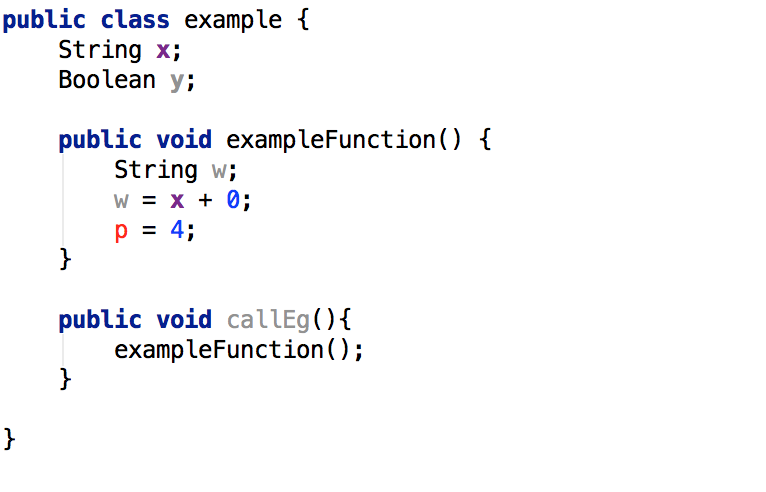
\includegraphics[width=0.50\textwidth]{jcode}
\caption{Example of Code Colouring}
\label{fig:jcode}
\end{figure}
The code in Figure~\ref{fig:jcode}, from Android Studio, shows some good examples of this. Global variables, which are variables that can be accesses from any part of the program as long as the call comes after the declaration, are coloured a separate colour. This requires some semantical analysis pre-compilation, as it is impossible to know whether a variable is global or not by syntactical analysis alone. The variable p is coloured red to indicate that it has not been declared yet, another useful feature. Variables that do not serve any function are coloured in grey, for example w in this example as its value is not used for anything. 

\end{itemize}



\section{Different Types Of Programming Language Used To Teach Beginners}\label{sec:teachL}

Easily the two most popular languages to teach programming with are Python and Java \cite{javapython}and there are a range of reasons for this. Both are high-level languages in that they hide much of the complexity, such as memory allocation and garbage collection, from the user. This makes it easier to teach than a lower level language such as C, which requires a deeper understanding of how computers interpret and run code. Whether this is a desirable feature of a language to be taught to beginners is a hot topic of debate, with many feeling that abstracting such aspects of programming at so early on in a programmers education means they will probably never learn about them and ultimately hinders their understanding and eventual capability as a programmer. However, opponents of this opinion would argue that this is a sacrifice worth making in order to flatten the learning curve for beginners. With UK schools already struggling on a shoestring budget to train their teachers to an adequate level to teach the children the new curriculum, expecting them to train their teachers to understand the ins and outs of C is unrealistic. 

Python has recently emerged as a fashionable choice for teaching programming as it is very concise compared to other languages, which can make it easier to understand. It dynamically typed, meaning that variables do not have to be declared with a name. The code below (Listing~\ref{lst:python}) would first output the \textbf{str} (Python's string type) ''hello'' then the \textbf{int} (Python's integer type) 2. Again, whether this is a good thing is debatable for the reasons outlined in the previous paragraph. 

\begin{quote}
\begin{lstlisting}[caption={Example Python code},label={lst:python},language=Python]
foo = "hello"
print foo
foo = 2
print foo
\end{lstlisting}
\label{lst:label}
\end{quote}

According to IEEE Spectrum, who each year publish a highly respected ranking of languages by popularity based on 12 metrics from 10 data sources (including the IEEE Xplore digital library, GitHub, and CareerBuilder), Java remains the most popular programming language in 2015, holding onto it's top sport for the second year running \cite{top}\. This, combined with the rising popularity of the Android mobile OS which runs on a version of Java, make it an attractive choice for many. It is strongly-typed, which means that once a variable has been assigned a type, it cannot be redeclared as a different type. For exmaple the code below (Listing~\ref{lst:java}) would return an error.

\begin{quote}
\begin{lstlisting}[caption={Example Java code},label={lst:java},language=Python]
String foo = ("hello");
System.out.println(foo);
Int foo = 2
System.out.println(foo);
\end{lstlisting}
\label{lst:label}
\end{quote}


Talk about history of language engineering, of real time error checking


Talk in depth how code block programming works

Talk in depth how code academy works

Talk in depth how CodeTouch meets in the middel

Talk about touch develop: sort of bridges gap but not quite, doesn't have flow of writing code like CodeTouch

talk about pencil code

Output is real code, looks like java but could be tweaked to be anything, or indeed to actually create valid java.


% -----------------------------------------------------------------------------

\chapter{Project Execution}
\label{chap:execution}

{\bf A topic-specific chapter, of roughly $20$ pages} 
\vspace{1cm} 



\section{Choice Between Developing A Native Application, Cross-Platform Application or Hybrid Application}
For CodeTouch, the performance of the application is very critical to the applications core function; when a user is generating code, it should feel as instant and natural as typing is on a computer. Seeing as it was difficult to predict if there would be any performance issues before development on the application started, the decision was made to go native in order to minimise the risk of poor performance affecting the application's use-ability. Once this decision was made, the decision to go for Android was made based on reasons articulated earlier in this document (see \ref{sec:Android}), plus I personally had more experience in Java than either Objective C or HTML5. (For an explanation of the three options see \ref{sec:ApTypes}).

\section{Choice of Integrated Development Environment}

When development for CodeTouch started there was a genuine choice between Eclipse and Android studio (see \ref{sec:andIDE}), as the Eclipse plugin was still being supported and developed, although there were suspicions of it's support being dropped as Android Studio had recently come out of beta mode. Having previously used Eclipse and with it already installed on my machine the temptation was there to stick with it, but ultimately Android Studio was chosen down to the fact that it's support was more guaranteed than Eclipse's.

\section{Layout}
There were many considerations I had to take into account when designing the layout for CodeTouch. One important decision was how big the menu would be. The only other similar application in terms of how the user enters code, TouchDevelop, has a very large, cluttered menu with 36 buttons on display at a time. I wanted to avoid this in order to leave as much space free for the code. 

\begin{figure}[h]
\centering
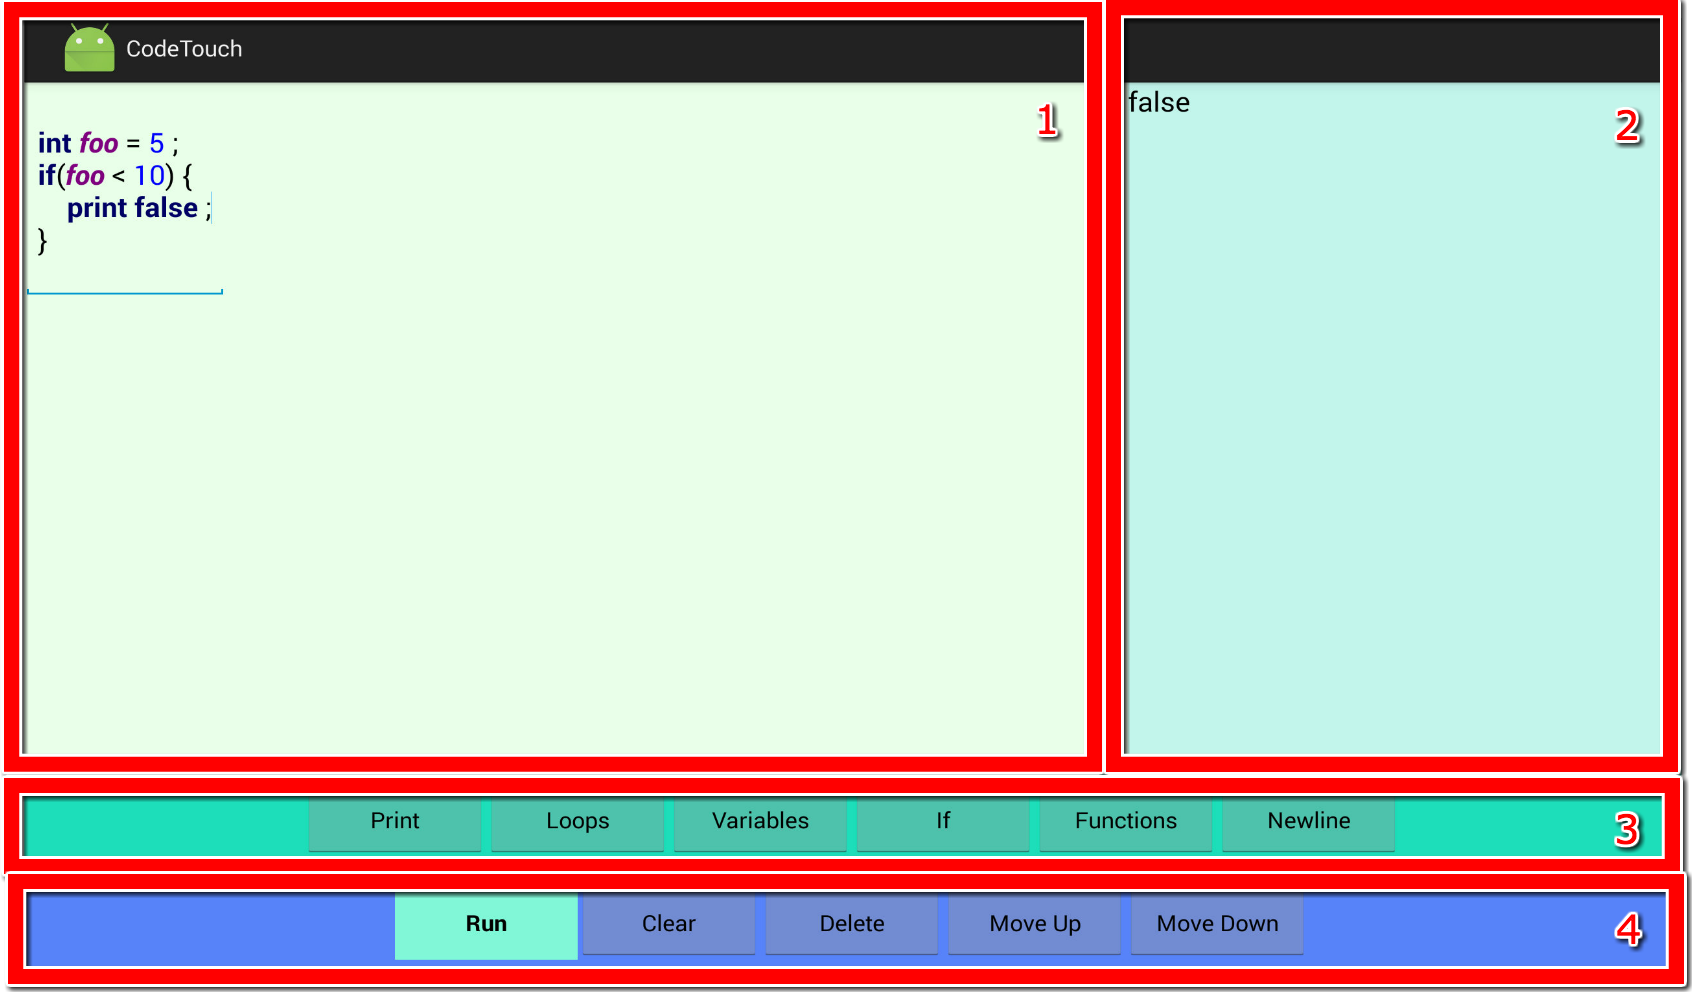
\includegraphics[width=0.80\textwidth]{UIN}
\caption{Graphical User Interface Appearance}
\label{fig:ui}
\end{figure}
`
Figure~\ref{fig:ui} shows my final design. As you can see, the majority of the screen is dominated the area labeled $1$, the code box.I made this decision based off responses to my initial survey (Question 5, ~\ref{ssec:survey}). There are two menu's at the bottom of the screen. The one labelled $3$ in the diagram is the code creation menu. It is dynamic in that the buttons on the menu change depending on the users current position in the program. The menu labelled $4$ is the control menu. This is where all the buttons for functions that do not add to the code reside. There is only one non-dynamic button, the run button. This button only appears when the code is in a valid, runnable state. 


\section{Designing the language}

\subsection{How much to restrict the user}
As laid out in my objectives, I wanted to create a programming environment where the user does not need to worry about semantic or syntactical mistakes. But there was some consideration to be made when implementing this. Just because I wanted the user to not have to worry about making mistakes didn't mean I wanted to completely stop them from making mistakes at all. People learn from making mistakes, and for this reason I identifed certain mistakes that I would allow users in CodeTouch to make. However, rather than let this mistake translate into the code, a pop-up box appears informing the user of their mistake.

\begin{figure}[h]
\centering
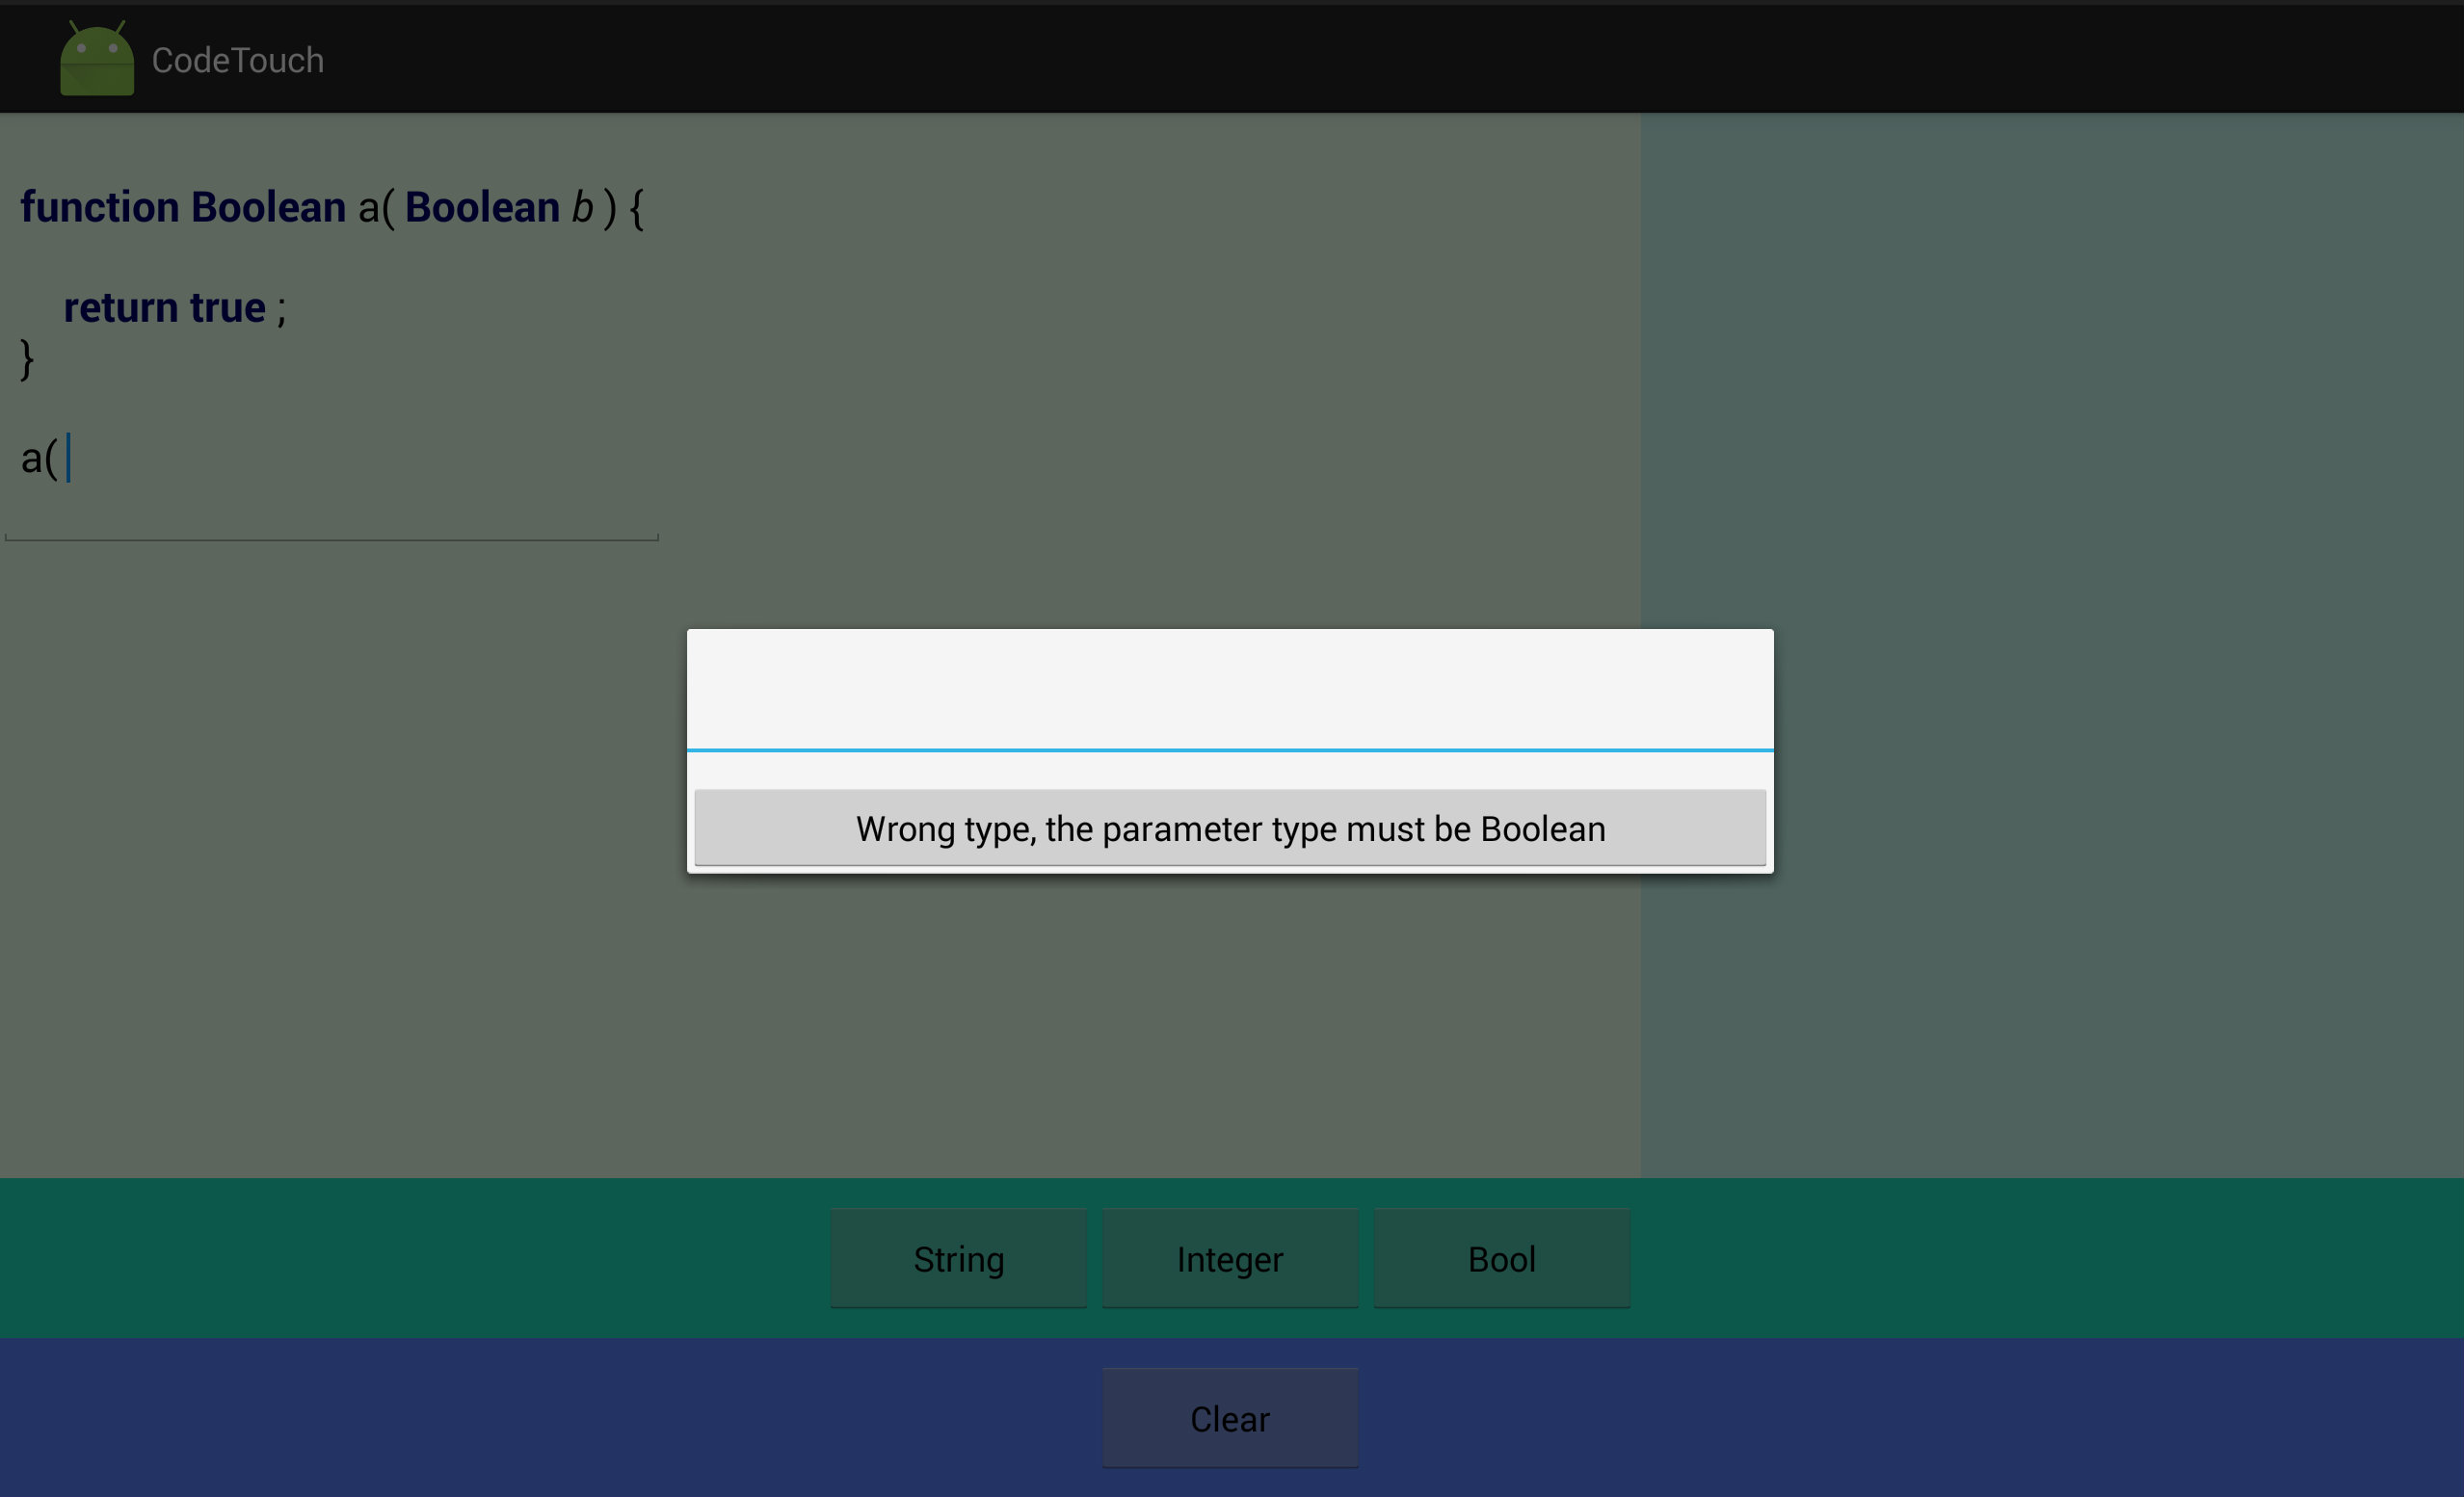
\includegraphics[width=0.80\textwidth]{boolmistake}
\caption{}
\label{fig:boolmistake}
\end{figure}

Figure~\ref{fig:boolmistake} shows what happens if you try to send a String as a parameter to a function that takes an Integer as a parameter. 

Another consideration I had to make when deciding how to limit the user was the different kind of users CodeTouch is aimed at. For more experienced users, making a semantic mistake can be a desired option. For example, I could prevent the user from making the semantic mistake of deleting a variable declaration when that variable is used later on in the code. However, they may just want to move the declaration to somewhere else, and requiring the user to delete every instance of the said variable before letting them move the declaration would be very frustrating for the user in this scenario. At the same time I still wanted to consider novices who might not know what they are doing. As a compromise I decided to show a warning when a user attempts to delete a variable already in use later on, letting the user know that this will cause an error but letting them make it if they want to. If this variable is deleted, the code is not be runnable until the declaration has been restored (enforced by the hiding of the run button).


\subsection{Designing the User Interface and Compilation Process}

Earlier in the document I described the conventional process of compilation in detail \ref{compilation}. To briefly recap, the overall process is as follows:

\begin{enumerate}
\item User writes code
\item Compiler performs lexical analysis to determine if all the characters it has been provided with can be turned into valid tokens of the language through the process of tokenization. 
\item Compiler performs syntactic analysis to determine if the tokens generated in the previous step make sense structurally with eachtother by attempting to build a Concrete Syntax Tree from the tokens, using a Context-Free Grammar and associated set of rules. 
\item Compiler performs semantic analysis to determine if code makes sense, in that all the elements of the parse tree generated in the previous step make sense with eachother in context, as well as performing other semantic checks such as array-bound checking
\item Abstract Syntax Tree is created from Concrete Syntax Tree in order to optimise the tree for the machine that is going to run the code
\item Machine-readable code generated from Abstract Syntax Tree. 


\end{itemize}

The problem with this process for CodeTouch is that at the very first step, the user can write incorrect code. The aim of CodeTouch was to create a programming tool which didn't allow this. The result of this objective meant that stages 2,3 and 4 have to happen before the user enters any code, meaning that the traditional compilation pipeline would not be suitable for the project. 

\subsubsection{Pre-tokenization}

Even just preventing lexical errors would be practically impossible to implement with a keyboard input, as it would not be possible to detect whether a user has made a mistake until they have finished typing the word they are writing, invalidating the requirements I set for CodeTouch. Of course, one could map each valid token in a language to a different key, but this would be impractical and near on unusable. On a tablet however, by creating dynamic buttons that map to valid tokens, we can limit the input to just a set of buttons that correspond to these valid tokens, a process that I have called pre-tokenization.


\section{Tree Modification}
The next problem was how to ensure that only buttons would lead to syntactically and semantically correct code would be on display at any time. This required syntactical and semantical analysis of the existing code in order to know what options should be available for the next button press. Syntactical and semantical analysis is performed using a syntax tree which, as detailed in \ref{compilation} By analysing the tree, using a set of rules, it is possible to know what inputs are valid. The consequence of this is that we need to analyse the Sytax tree for the current source code every time we want to add a token to the code. Traditionally, the tree is usually built from the source code using some kind of grammar (see \ref{contextfreegrammar}). One approach that could have been taken at this stage would have been to rebuild the tree from the source code every time a button is pressed, which would result in some rather hefty computation. This approach would have a sever impact on the performance of the application, especially once the program starts to grow in size.The logical solution to this is to keep the tree stored in memory and make incremental modifications as the user builds up their program.

These modifications could be done from analysing the text just added to the source code, but this would be a naive approach as it would then require lexical analysis to tokenize the text, which would not take advantage of the fact that the tokenization has, in effect, already been done by only allowing the user to add valid tokens to the text. 

Another approach would be to simultaneously add the text to the source code and modify the tree. However, is it not difficult to imagine the difficulties that could arise in trying to make sure that the text and the tree stay in sync, especially when moving around the program and changing things.

The third option was to make the button presses directly modify the tree, then build the code backwards from the tree. Although this method does require a single pass through the tree after each button press, it us computationally much cheaper than building the tree from the source code after each button press and makes it much easier to maintain as the problem of keeping the code and the tree in sync becomes a non-issue. For these reasons I chose this approach. This process is illustrated in Figure~\ref{processes}.



\begin{figure}[h]
\centering
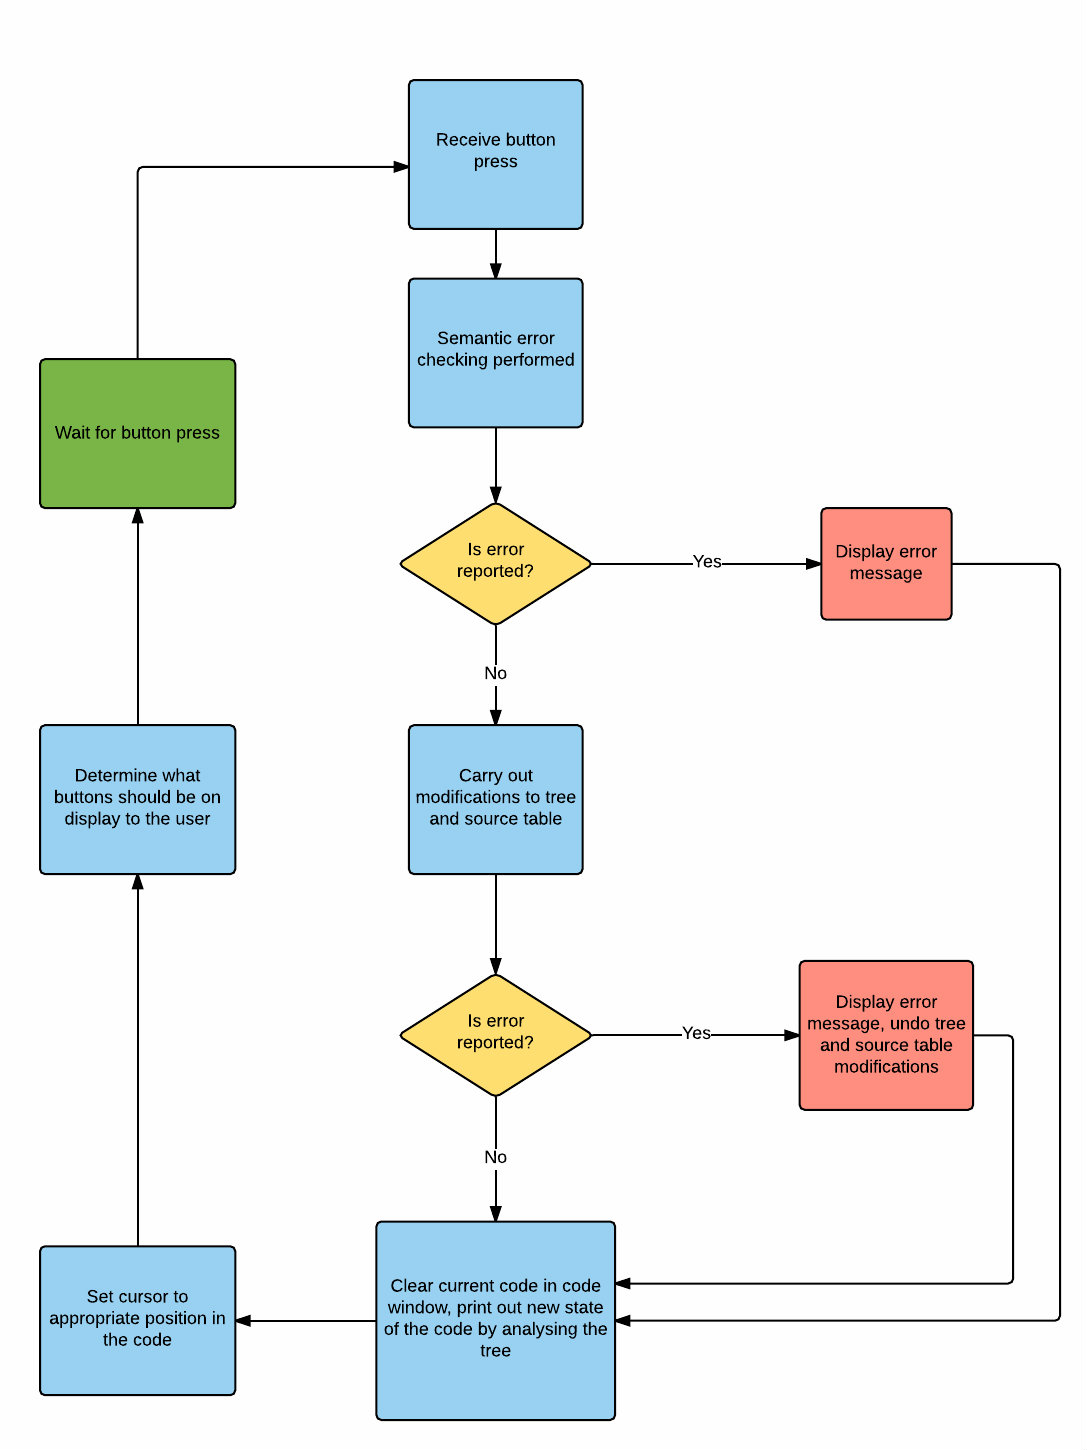
\includegraphics[width=0.80\textwidth]{process}
\caption{CodeTouch's Compilation Process}
\label{fig:processes}
\end{figure}

\subsubsection{Running the Code}

A consequence of building the tree as we go along is that we do not need to compile the code in order to run it, as it has essentially been incrementally compiled as it was being produced, meaning that it is possible to run the code instantly (Note: in CodeTouch you can only run the program once the code is in a runnable state). However, a side-effect of the decision to produce the code backwards from the tree meant that the tree itself has to be an exact representation of the code, making it what is known as a Concrete Syntax Tree. Concrete Syntax trees contain many nodes which are unnecessary for a computer to understand the semantics of the code, and the usual process is to convert the tree to an Abstract Syntax Tree and optimise it as much as possible (see \ref{ssec:icm}) before converting it into machine-readable text. One option would have been to create an optimal Abstract Syntax Tree from the Concrete Syntax Tree whenever the user runs the code, and for long, complex programs this certainly would speed up the run time. However, CodeTouch's main target audience at this stage of development is beginners, so the programs that would be created are unlikely to be very complex; these types of program run very quickly on the application and as such optimising it further was not a priority. However, it is a feature that is planned for future development. 


\section{Implementing the language}


The solution to this was to limit the input options so that only 

In my case the machine that had to read it was Java.

impossible to make syntactially incorrect code. Also semantically to an extent: ie can't use a variable that has not been declared, if you delete definition when it is usesd later it gives you a warning. 



\section{Appearance of the language}
When using CodeTouch, the user never really see's what the code they are making looks like, as they build the language tree directly, which is then analysed to produce the code afterwards. This meant that I could choose how the code would be displayed to the user, and indeed change this easily without having to redefine the language. 

The two most popular languages to teach programming in are Java and Python (see \ref{sec:teachL}). For the language to be used in CodeTouch I decided to make it look more like Java, as this results in more verbose code, which suits CodeTouch as this results in there being less disparity between button presses and code appearing on the screen. The process of declaring a variable illustrates this point well. Because CodeTouch is designed to use the keyboard as little as possible, when declaring a variable it is necessary that the user is prompted to press a button to choose the type of the variable before naming it, as this then dictates which buttons will be visible for the rest of that line of code (for example, if a Boolean is chosen then the operators menu will bring up a different set of operators when clicked than if a String had been chosen). At this point in a statically-typed language, the name of the selected type will be output to the screen, for example:
 
\begin{quote}
\begin{lstlisting}[caption={Output when Boolean type is selected for variable declaration in Java},label={lst:javaDec},language=Java]
Boolean
\end{lstlisting}
\label{lst:label}
\end{quote}

If I had chosen to make it dynamically typed, I still would have had to require that the user press this button so as to avoid requiring the user to have to type in quote marks when entering it's value (which is undesirable as I want to use the keyboard as little as possible). This would not result in any text being added to the code and would thus disrupt the flow and feel of the process. 


\noindent
This chapter is intended to describe what you did: the goal is to explain
the main activity or activities, of any type, which constituted your work 
during the project.  The content is highly topic-specific, but for many 
projects it will make sense to split the chapter into two sections: one 
will discuss the design of something (e.g., some hardware or software, or 
an algorithm, or experiment), including any rationale or decisions made, 
and the other will discuss how this design was realised via some form of 
implementation.  

This is, of course, far from ideal for {\em many} project topics.  Some
situations which clearly require a different approach include:

\begin{itemize}
\item In a project where asymptotic analysis of some algorithm is the goal,
      there is no real ``design and implementation'' in a traditional sense
      even though the activity of analysis is clearly within the remit of
      this chapter.
\item In a project where analysis of some results is as major, or a more
      major goal than the implementation that produced them, it might be
      sensible to merge this chapter with the next one: the main activity 
      is such that discussion of the results cannot be viewed separately.
\end{itemize}

\noindent
Note that it is common to include evidence of ``best practice'' project 
management (e.g., use of version control, choice of programming language 
and so on).  Rather than simply a rote list, make sure any such content 
is useful and/or informative in some way: for example, if there was a 
decision to be made then explain the trade-offs and implications 
involved.

\section{Future Development}
There are many features that were planned but did not get implemented in the alloted time for the project. 
\begin{enumerate}
\item Although not yet implemented, CodeTouch's interface is designed to accommodate a similar challenge-based lesson system.
\item Finish the editing capabilities
\item More programming functionailty - arrays 
\item Optimise runtime by creating abstract syntax tree (ie do reverse polish notation)
\item Ability to program in real languages - easy, why?
\item Ability to export programs as executable code in these languages. This would turn concrete syntax tree into abstract syntax tree and optimise first. The ability to do this could also be useful for a "fast run" option, where AST is compiled. 
\end{enumerate}



\chapter{Critical Evaluation}
\label{chap:evaluation}

{\bf A topic-specific chapter, of roughly $10$ pages} 
\vspace{1cm} 

\noindent

\section{Comparison with Competiton}
\subsection{CodeTouch vs Scratch}
As mentioned previously (see ~\ref{ssec:Scratch}), Scratch is a code-block visual language. 

Although it is great for what it does, it is not a direct competitor of CodeTouch as it is aimed at a much younger audience, and the drag and drop method of producing code does not reproduce the feel and flow of type based coding, which my user-testing shows that CodeTouch successfully achieves. 

\subsection{CodeTouch vs CodeAcademy}

CodeAcademy is, as outlined earlier in this document, CodeAcademy is a typing-based web application (see \ref{ssec:CodeAcademy}. While there are many positive aspects of CodeAcademy that have inspired CodeTouch, CodeTouch improves on CodeAcademy in a number of ways. In CodeTouch, the intelligent error reporting happens in real time, without the need for compiling the code, pointing out errors to users as they are making them, as opposed to CodeAcademy which only reports errors after compilation. Furthermore, CodeAcademy is a web application and whilst it can be accessed from a tablets browser, it does not take advantage of any aspects of the touchscreen. 

Although CodeAcademy has so far been popular in schools, it does not directly address the problem of the transition from visual code-block languages to textual languages that CodeTouch aims to solve, as it is not a syntax and semantic-mistake free environment, giving CodeTouch an edge in this respect.


\subsection{CodeTouch vs TouchCode}
TouchDevelop is Microsoft's touch-based coding tool (see \ref{ssec:TD}). It is CodeTouch's most similar rival, but CodeTouch improves on it's in some key areas. The back and forth screen presses between the menu and the code required to perform simple processes such as variable declaration is an area that CodeTouch improves on significantly; in CodeTouch the user can write a whole program without moving their fingers from the menu. For example, to program the code in Listing\ref{lst:varcode} takes requires the user to leave the menu [X] times, with [X] screen presses, while the same process on CodeTouch doesn't require the user to press anywhere except the menu and takes [X] screen presses. 

CodeTouch is also provides a syntax error and semantic error free environment which TouchDevelop does not provide, which my user feedback showed was a much appreciated feature of CodeTouch \ref{SURVRERRTY}.

\section{The Language}
In CodeTouch, the language tree is constructed directly from the button presses, with the code being assembled from this afterwards. The result of this is that it makes it very easy to change how the code that is produced looks to the user. The advantage of this is that it would be very easy to make the code output become a subset of a real language. For example, although in it's current form the outputted code is a custom language designed to be easy to understand by beginners, it could easily be modified to output Java or Python code without much of the actual language being changed.

\begin{quote}
\begin{lstlisting}[label={lst:python},language=Python]
String x = "hello";
String y = "world";
x = x + y;
\end{lstlisting}
\label{lst:label}
\end{quote}

Although this may not be of as much significance to complete beginners, it is an attractive improvement for more experienced coders using CodeTouch, as articulated by the subjects of my user-feedback sessions [ADD REFERENCE].

TouchCode also is not a syntax-mistake free environment, making it less nurturing than CodeTouch, although it does have a strong real time error reporting system.








This chapter is intended to evaluate what you did.  The content is highly 
topic-specific, but for many projects will have flavours of the following:

TALK ABOUT how i could have used reverse shunting algorithm for brackets expression, explain it in depth

IDEA colaberative programming for classroom, so every pupil could have tablet with code, teacher chooses person to do next line

\begin{enumerate}
\item functional  testing, including analysis and explanation of failure 
      cases,
\item behavioural testing, often including analysis of any results that 
      draw some form of conclusion wrt. the aims and objectives,
      and
\item evaluation of options and decisions within the project, and/or a
      comparison with alternatives.
\end{enumerate}



\noindent
This chapter often acts to differentiate project quality: even if the work
completed is of a high technical quality, critical yet objective evaluation 
and comparison of the outcomes is crucial.  In essence, the reader wants to
learn something, so the worst examples amount to simple statements of fact 
(e.g., ``graph X shows the result is Y''); the best examples are analytical 
and exploratory (e.g., ``graph X shows the result is Y, which means Z; this 
contradicts , which may be because I use a different assumption'').  As 
such, both positive {\em and} negative outcomes are valid {\em if} presented 
in a suitable manner.

% -----------------------------------------------------------------------------

\chapter{Conclusion}
\label{chap:conclusion}

{\bf A compulsory chapter, of roughly $2$ pages} 
\vspace{1cm} 

\noindent
The concluding chapter of a dissertation is often underutilised because it 
is too often left too close to the deadline: it is important to allocation
enough attention.  Ideally, the chapter will consist of three parts:

talk about how code colouring

\begin{enumerate}
\item (Re)summarise the main contributions and achievements, in essence
      summing up the content.
\item Clearly state the current project status (e.g., ``X is working, Y 
      is not'') and evaluate what has been achieved with respect to the 
      initial aims and objectives (e.g., ``I completed aim X outlined 
      previously, the evidence for this is within Chapter Y'').  There 
      is no problem including aims which were not completed, but it is 
      important to evaluate and/or justify why this is the case.
\item Outline any open problems or future plans.  Rather than treat this
      only as an exercise in what you {\em could} have done given more 
      time, try to focus on any unexplored options or interesting outcomes
      (e.g., ``my experiment for X gave counter-intuitive results, this 
      could be because Y and would form an interesting area for further 
      study'' or ``users found feature Z of my software difficult to use,
      which is obvious in hindsight but not during at design stage; to 
      resolve this, I could clearly apply the technique of Smith [7]'').
\end{enumerate}

% =============================================================================

% Finally, after the main matter, the back matter is specified.  This is
% typically populated with just the bibliography.  LaTeX deals with these
% in one of two ways, namely
%
% - inline, which roughly means the author specifies entries using the 
%   \bibitem macro and typesets them manually, or
% - using BiBTeX, which means entries are contained in a separate file
%   (which is essentially a databased) then inported; this is the 
%   approach used below, with the databased being dissertation.bib.
%
% Either way, the each entry has a key (or identifier) which can be used
% in the main matter to cite it, e.g., \cite{X}, \cite[Chapter 2}{Y}.

\backmatter

\bibliography{dissertation}


% -----------------------------------------------------------------------------

% The dissertation concludes with a set of (optional) appendicies; these are 
% the same as chapters in a sense, but once signaled as being appendicies via
% the associated macro, LaTeX manages them appropriatly.

\appendix

\chapter{An Example Appendix}
\label{appx:example}



Content which is not central to, but may enhance the dissertation can
be included in one or more appendices; examples include, but are not 
limited to

\begin{itemize}
\item lengthy mathematical proofs, numerical or graphical results
      which are summarised in the main body,
\item sample or example calculations, 
      and
\item results of user studies or questionnaires.
\end{itemize}


\noindent
Note that in line with most research conferences, the marking panel 
is not obliged to read such appendices.

% =============================================================================
\subsection{Survey Results}
\label{ssec:survey}
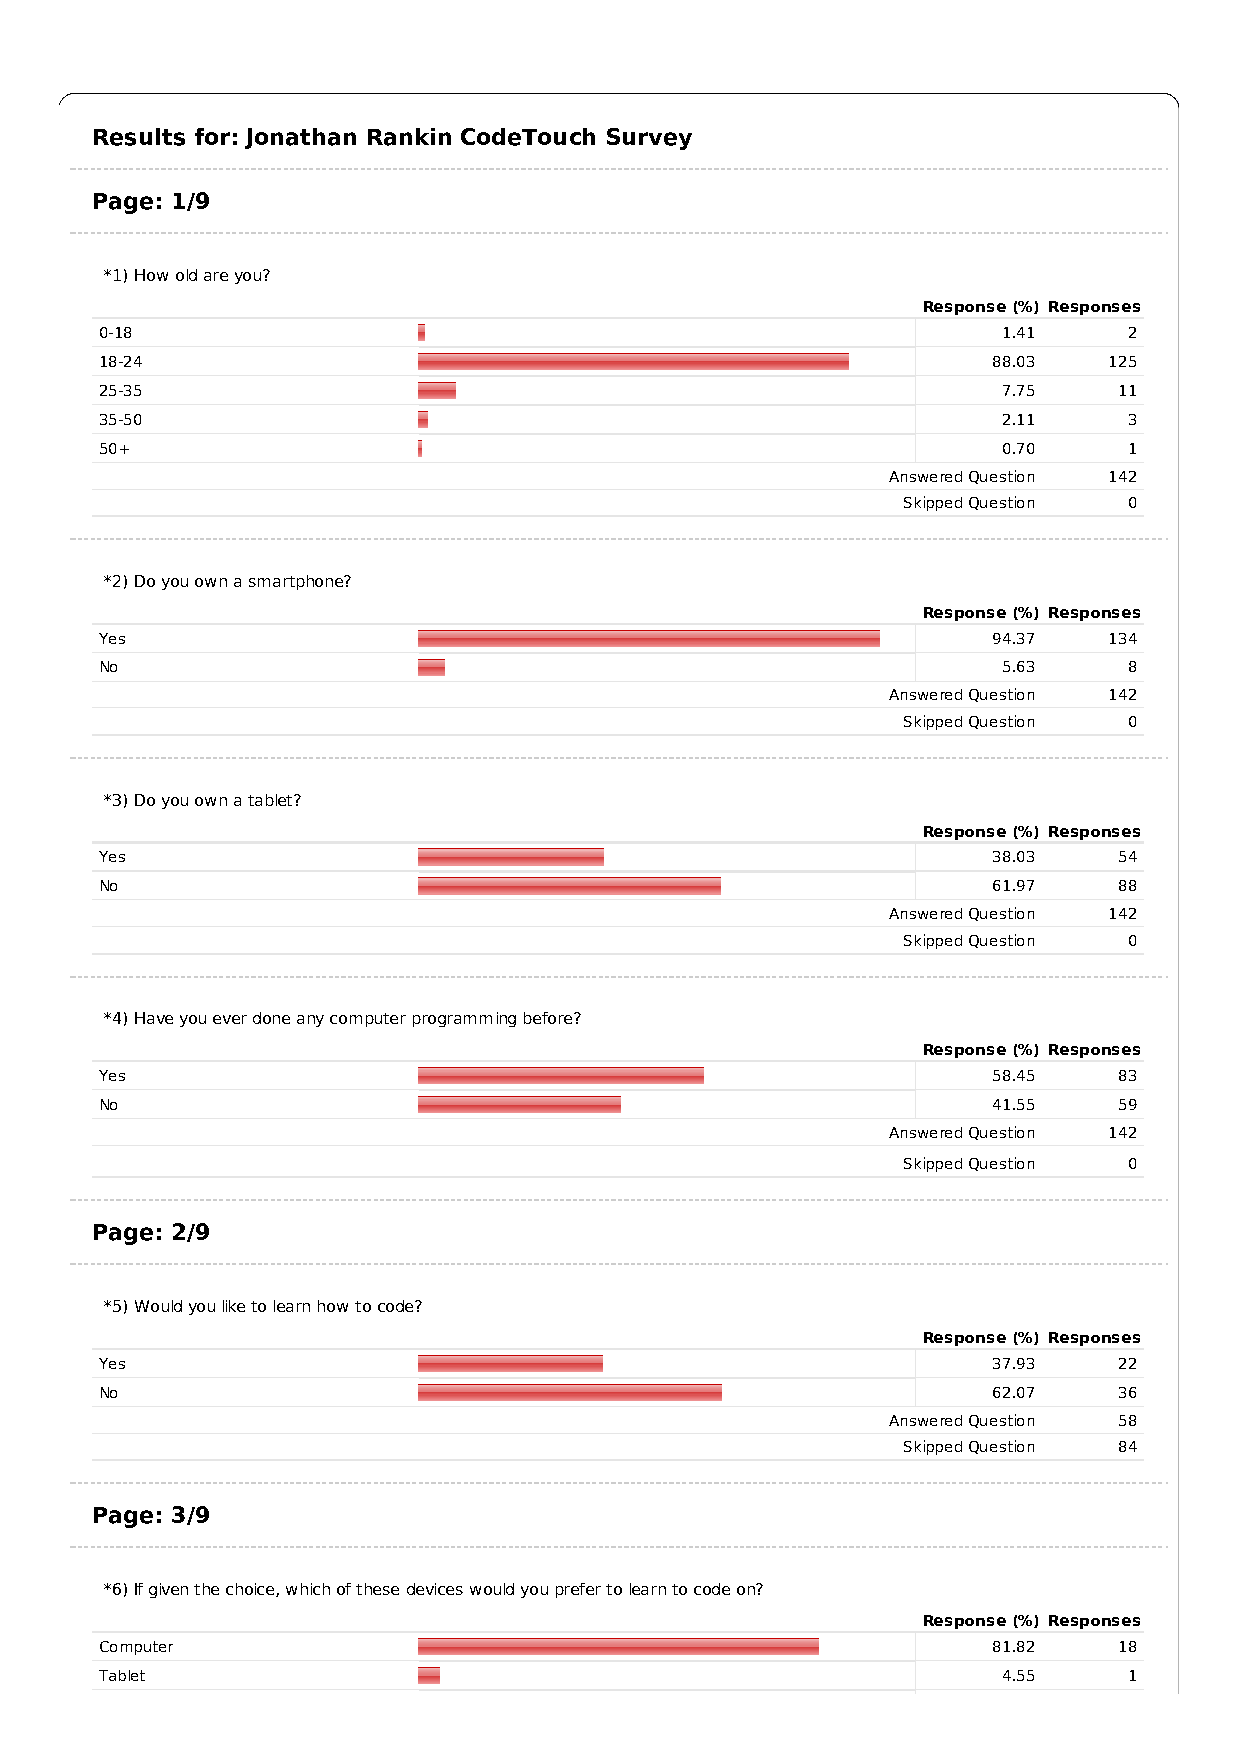
\includepdf[pages={1-6}]{survey.pdf}

\end{document}
